\documentclass{article}

\usepackage{amsmath}
\usepackage{amsthm}
\usepackage{amssymb}
\usepackage{amsfonts}
\usepackage{mathtools}

\usepackage{arxiv/arxiv}
\usepackage{styles/quiver}

\usepackage[utf8]{inputenc} % allow utf-8 input
\usepackage[T1]{fontenc}    % use 8-bit T1 fonts
\usepackage{hyperref}       % hyperlinks
\usepackage{url}            % simple URL typesetting
\usepackage{booktabs}       % professional-quality tables
\usepackage[english]{babel}
\usepackage{nicefrac}       % compact symbols for 1/2, etc.
\usepackage{microtype}      % microtypography
\usepackage{graphicx}
\usepackage{stmaryrd}

\usepackage{tikz}
\usetikzlibrary{angles,fit,arrows,calc,math,intersections,through,backgrounds}
\usepackage{qtree}

\usepackage{listings}
\lstset{
  basicstyle=\itshape,
  xleftmargin=3em,
  literate={->}{$\rightarrow$}{2}
           {α}{$\alpha$}{1}
           {δ}{$\delta$}{1}
}

\usepackage{xstring}
\usepackage{stmaryrd}
\usepackage{wasysym}
\usepackage{textcomp}
\usepackage{blindtext}
\usepackage{subfiles}

\newtheorem{definition}{Definition}
\numberwithin{definition}{section}
\newtheorem{lemma}{Lemma}
\numberwithin{lemma}{section}
\newtheorem{proposition}{Proposition}
\numberwithin{proposition}{section}
\newtheorem{corollary}{Corollary}
\numberwithin{corollary}{section}
\newtheorem{theorem}{Theorem}
\numberwithin{theorem}{section}

\DeclareMathSymbol{\mathinvertedexclamationmark}{\mathclose}{operators}{'074}
\DeclareMathSymbol{\mathexclamationmark}{\mathclose}{operators}{'041}
\makeatletter
\newcommand{\raisedmathinvertedexclamationmark}{%
  \mathclose{\mathpalette\raised@mathinvertedexclamationmark\relax}%
}
\newcommand{\raised@mathinvertedexclamationmark}[2]{%
  \raisebox{\depth}{$\m@th#1\mathinvertedexclamationmark$}%
}
\begingroup\lccode`~=`! \lowercase{\endgroup
  \def~}{\@ifnextchar`{\raisedmathinvertedexclamationmark\@gobble}{\mathexclamationmark}}
\mathcode`!="8000
\makeatother

\DeclareMathOperator{\arcsinh}{arcsinh}
\DeclareMathOperator{\Tr}{Tr} % Example, if trace was needed

\title{Geometry of Arithmetic Expressions: I.\\ Basic Concepts and Unsolved Problems (Draft)}

%\date{Decmber 8, 2022}	% Here you can change the date presented in the paper title
%\date{} 				% Or removing it

\author{
Mingli Yuan \\
Swarma Research\\
Beijing, 100083 \\
\texttt{mingli.yuan@gmail.com}
}

% Uncomment to remove the date
%\date{}

% Uncomment to override  the `A preprint' in the header
\renewcommand{\headeright}{A preprint}
\renewcommand{\undertitle}{A preprint}

\begin{document}
\maketitle

\begin{abstract}
    This paper introduces a novel geometric framework for studying arithmetic expressions, establishing a rigorous connection between algebraic operations and hyperbolic geometry. We formalize arithmetic expressions as syntactic structures and demonstrate how they can be embedded into continuous geometric spaces where addition and multiplication correspond to movements along orthogonal directions. Central to our approach is a flow equation that governs how expression values propagate through this geometric space. We construct the first kind arithmetic expression space $\mathfrak{E}_1$ on the upper half-plane with a hyperbolic metric, where the assignment function satisfies the flow equation and serves as an eigenfunction of the Laplacian. This construction reveals that arithmetic torsion—the non-commutativity of addition and multiplication—directly corresponds to geometric area, analogous to how curvature measures deviation from flatness. The paper establishes arithmetic expressions as geometric objects with intrinsic invariants, opening new avenues for exploring the interplay between computation and geometry.
\end{abstract}

\keywords{arithmetic expressions, hyperbolic geometry}

\setcounter{tocdepth}{2}
\tableofcontents
\newpage

\section{Introduction}\label{sec:introduction}

Can arithmetic expressions form a geometric space?
In this paper, we present several examples of arithmetic expression spaces and examine their properties.

TODO

\newpage

\section{Basic concepts}\label{sec:concepts}

%! suppress = UnresolvedReference
% \usepackage{amsfonts}
% \usepackage{amsmath}
% \usepackage{graphicx}
% \usepackage{mathtools}

\subsection{Arithmetic expression}\label{sec:expression}

In order to define arithmetic expressions involving real numbers  $\mathbb{R}$ in a rigorous way, we need to use a sophisticated type theory.
However, in order to keep things simple and maintain clarity, we will start by using only production rules, but with certain semantic restrictions.
We will also begin with rational numbers $\mathbb{Q}$ to avoid the difficulties inside real numbers $\mathbb{R}$ .

\begin{definition}\label{def:arithmetic-expression}
    An arithmetic expression $a$ over $\mathbb{Q}$ is a structure given by the following production rules:
\begin{equation}\label{eq:productionrule}
\begin{aligned}
a &\longleftarrow x\\
a &\longleftarrow ( a + a )\\
a &\longleftarrow ( a - a )\\
a &\longleftarrow ( a \times a )\\
a &\longleftarrow ( a \div a )
\end{aligned}
\end{equation}
    where $x \in \mathbb{Q}$, and we denote this as $a \in \mathbb{E} \left [\mathbb{Q} \right ]$.
\end{definition}

During the production process, we can obtain both a string representation and a tree representation of arithmetic expression $a$,
where the two representations are equivalent.
For instance, the string representation of $a$ might be:

\begin{equation}
(((((1 \times 2) \times 2) - 1) \times (2 + 1)) - 6)\label{eq:equation}
\end{equation}

and the parsed syntax tree is depicted in Figure~\ref{fig:syntaxtree}.

\begin{figure}[ht]
\centering
\resizebox{0.2\textheight}{!}{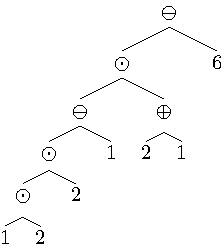
\includegraphics{images/02-example-expression-syntax-tree.pdf}}
\caption{a tree representation of an arithmetic expression}\label{fig:syntaxtree}\label{fig:figure}
\end{figure}

If we interpret the target as a string and the building processes in production rule~\eqref{eq:productionrule} as string building, we get the \emph{string representation}.
On the other hand, if the target is a tree, tree building leads to the \emph{tree representation}.
We can easily obtain the string representation of $a$ from its tree representation by performing a pre-order traversal.

The concept of a \emph{sub-expression} can also be derived from the concept of a subtree.
The branch nodes are all labeled with operators: $+$, $-$, $\times$, $\div$.
The leaf nodes are all labeled with numbers.

Evaluation $\nu$ is a partial function that operates on arithmetic expression $a \in \mathbb{E} \left [\mathbb{Q} \right ]$.
It is undefined only if division by zero occurs during the recursive evaluation process.

We can define evaluation $\nu(a)$ of $a$ recursively as follows:
\begin{itemize}
  \item Constant leaf: for any $x \in \mathbb{Q}$, $\nu(x) = x$.
  \item Compositional node by $+$: For any $(a + b)$, $\nu((a + b)) = \nu(a) + \nu(b)$.
  \item Compositional node by $-$: For any $(a - b)$, $\nu((a - b)) = \nu(a) - \nu(b)$.
  \item Compositional node by $\times$: For any $(a \times b)$, $\nu((a \times b)) = \nu(a) \nu(b)$.
  \item Compositional node by $\div$: For any $(a \div b)$, if $\nu(b) \neq 0$, then $\nu((a \div b)) = \nu(a) / \nu(b)$.
\end{itemize}

We say that an arithmetic expression $a$ is \emph{evaluable} if $\nu(a)$ is defined.
In the rest of this article, we will only consider evaluable arithmetic expressions unless stated otherwise.

Given an arithmetic expression $a$, whatever evaluable or not, we can obtain its tree representation.
If a node $l$ is a leaf node, its corresponding subexpression $s$ is a number, so we consider it to be already \("\)evaluated\("\).
If a node $b$ is a branch node, its corresponding subexpression $s$ is an expression, and we can apply $\nu$ to it to obtain a number $\nu(s)$.
During the recursive evaluation process, starting from the leaves and moving towards the root, the subexpressions are evaluated one after another.
However, the order of evaluations is generally not unique.

\begin{definition}
The evaluation order of an arithmetic expression $a$ is an ordering of branch nodes in the tree representation of $a$
such that every node (sub-expression) is evaluated before its parent.
\end{definition}

For example, the possible evaluation orders of the arithmetic expression in Figure~\ref{fig:syntaxtree} are:
\begin{itemize}
  \item $1 \times 2 \rightarrow \underline{2}; \underline{2} \times 2 \rightarrow \underline{4}; \underline{4} - 1 \rightarrow \underline{3}; 2 + 1 \rightarrow \underline{3}; \underline{3} \times \underline{3} \rightarrow \underline{9}; \underline{9} - 6 \rightarrow 3$
  \item $1 \times 2 \rightarrow \underline{2}; \underline{2} \times 2 \rightarrow \underline{4}; 2 + 1 \rightarrow \underline{3}; \underline{4} - 1 \rightarrow \underline{3}; \underline{3} \times \underline{3} \rightarrow \underline{9}; \underline{9} - 6 \rightarrow 3$
  \item $1 \times 2 \rightarrow \underline{2}; 2 + 1 \rightarrow \underline{3}; \underline{2} \times 2 \rightarrow \underline{4}; \underline{4} - 1 \rightarrow \underline{3}; \underline{3} \times \underline{3} \rightarrow \underline{9}; \underline{9} - 6 \rightarrow 3$
  \item $2 + 1 \rightarrow \underline{3}; 1 \times 2 \rightarrow \underline{2}; \underline{2} \times 2 \rightarrow \underline{4}; \underline{4} - 1 \rightarrow \underline{3}; \underline{3} \times \underline{3} \rightarrow \underline{9}; \underline{9} - 6 \rightarrow 3$
\end{itemize}

The underlined numbers are the numbers that are evaluated during the evaluation process.

Below are examples of expressions that have a unique evaluation order.
These include right-expanded, left-expanded,
and combinations of them, as shown in Figure~\ref{fig:leftright} and Figure~\ref{fig:combination}.

\begin{figure}[ht]
\centering
\resizebox{0.4\textheight}{!}{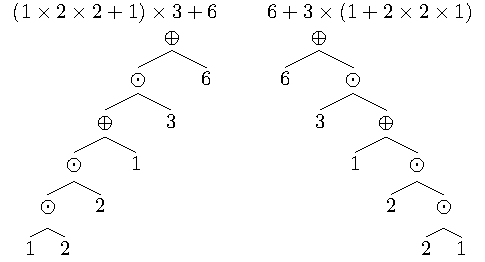
\includegraphics{images/03-example-expression-syntax-tree-left-right.pdf}}
\caption{right-expanded and left-expanded expressions}\label{fig:leftright}
\end{figure}

\begin{figure}[ht]
\centering
\resizebox{0.2\textheight}{!}{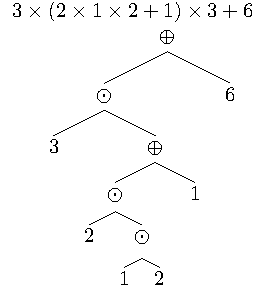
\includegraphics{images/04-example-expression-syntax-tree-combination}}
\caption{combinations of right-expanded and left-expanded expressions}\label{fig:combination}
\end{figure}

The evaluation order of an arithmetic expression is related to the topological order of its tree representation, but they are not the same.
The topological order of a tree is an ordering of nodes such that every node is visited before its parent\cite{Knuth1997TheAO}.
However, we are only interested in the ordering of branch nodes, as leaf nodes have already been evaluated and can be ignored.
Additionally, the topological order goes from parent to children, while the evaluation order goes from children to parent.

\begin{definition}
A threadlike expression is an arithmetic expression that all the left nodes in its tree representation are leaf nodes.
\end{definition}

So a threadlike expression is right-expanded and its evaluation order is unique.
One example of threadlike expressions is shown on the left side of Figure~\ref{fig:leftright}.

Threadlike expressions are significant here because they are analogous to the concept of paths in homotopy theory in geometry.
In a more general context, certain special types of threadlike expressions are also interesting:
for example, \emph{alternating threadlike expressions} are expressions in which the additional and multiplicative operators appear in an alternating manner.
In the field of computing, a hardware component called \emph{multiplier-accumulator} (MAC) unit has been implemented~\cite{Quinnell2007FloatingPointFM},
which is a special case of an alternating threadlike expression.
As a result, some numerical algorithms based on MAC units have been studied~\cite{Markstein2004SoftwareDA}.

\subsection{A scalar field and a mesh grid}\label{subsec:meshgrid}

Consider the upper half plane $\{\mathcal{H}: (x, y) | y > 0 \}$ equipped with an inner product and metrics defined as follows:

\[
\mathbf{a} \cdot \mathbf{b} = \begin{bmatrix} a_x & a_y \end{bmatrix} \begin{bmatrix} \frac{1}{y^2} & 0 \\ 0 & \frac{1}{y^2 \ln^2 2} \end{bmatrix} \begin{bmatrix} b_x \\ b_y \end{bmatrix}
\]

and

\[
ds^2 = \frac{1}{y^2} (dx^2 + \frac{dy^2}{\ln^2 2})
\]

We consider a scalar field satisfying

\begin{equation}
A = - \frac{x}{y}\label{eq:assignment}
\end{equation}

We call this field an \emph{assignment}.

Proper assignments allow us to establish a connection between paths in homotopy and threadlike arithmetic expressions,
and to incorporate function theory into the study of arithmetic expression geometry.

\begin{figure}[ht]
\centering
\resizebox{0.9\textwidth}{!}{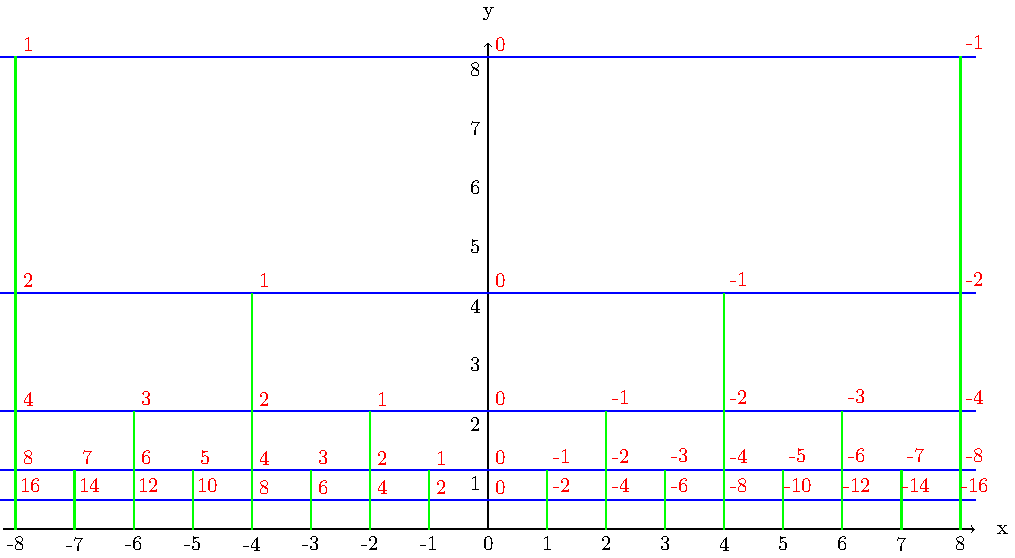
\includegraphics{images/01-grid-example-1.pdf}}
\caption{An addition-multiplication grid by generators with $\mu=1$ and $\lambda=\ln 2$}\label{fig:gridex0}
\end{figure}

We can draw a grid on the scalar field $A$ and underlying upper half plane $\mathcal{H}$ as shown in Figure~\ref{fig:gridex0}.
The blue lines encode a $+ 1$ relationship, the green lines encode a $\times 2$ relationship,
and they are line families that are perpendicular to each other.
The length of the line segments between two neighboring crossing points are unit length(calculations in lemma~\ref{lem:regular}).
The red value at the crossing points is the value of the scalar field $A$ at that point.
Based on the relationships encoded by the lines, we can encode threadlike arithmetic expressions,
which will be introduced in the subsection~\ref{subsec:encoding}.

The addition-multiplication grid is also scale-invariant under the transformation
\[
\begin{cases}
x' = \alpha x\\
y' = \alpha y
\end{cases}
\]

where $\alpha = 2^k , k \in \mathbb{Z}$.

We can image if we make the grid finer and finer, the grid will become a continuous space.
This leads to a rigorous treatment of arithmetic expressions as a geometric space in section~\ref{sec:topology}.

\subsection{Encoding threadlike expressions on the addition-multiplication grid}\label{subsec:encoding}

If we interpret the horizontal blue lines as $+ 1$ and the vertical green lines as $\times 2$ in Figure~\ref{fig:gridex0},
we can encode threadlike expressions on the addition-multiplication grid.
For example, in Figure~\ref{fig:encoding}
we encode $((((1 \times 4) - 1) \times 2) - 3)$ as the bold black lines.

\begin{figure}[ht]
\centering
\resizebox{0.9\textwidth}{!}{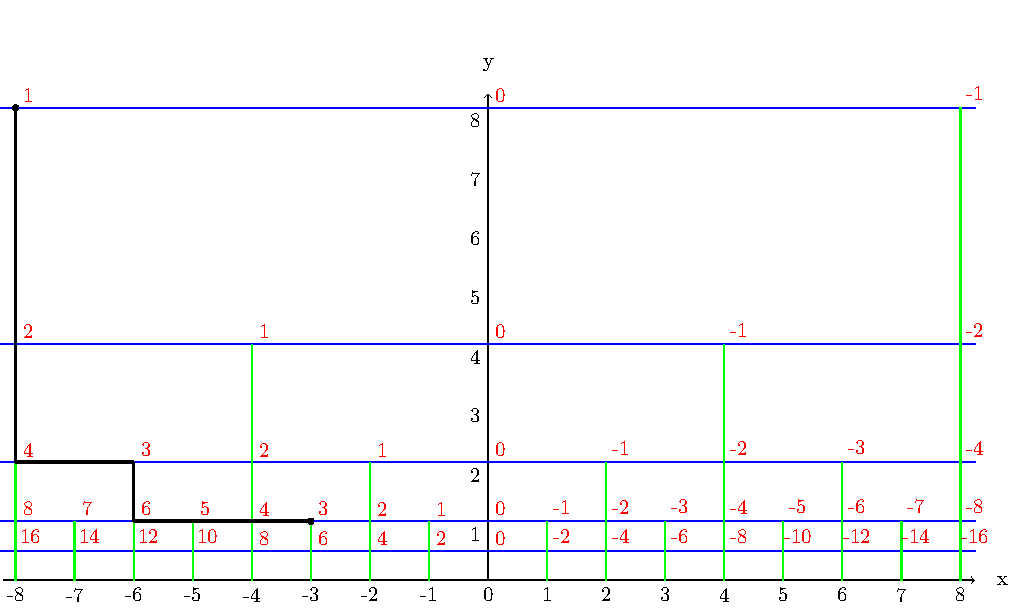
\includegraphics{images/05-example-expression-embedding}}
\caption{encoding threadlike expression}\label{fig:encoding}
\end{figure}

The zigzag lines in Figure~\ref{fig:encoding} can be divided into four parts:
\begin{itemize}
\item the vertical line from $1$ to $4$: encoded as multiplication by $4$
\item the horizontal line from $4$ to $3$: encoded as subtraction by $1$
\item the vertical line from $3$ to $6$: encoded as multiplication by $2$
\item the horizontal line from $6$ to $3$: encoded as subtraction by $3$
\end{itemize}

\subsection{From a scalar field to a space of threadlike expressions}\label{subsec:from-field-to-space}

As shown in Figure~\ref{fig:canonicalform}, we have the following paths and expressions:
\begin{itemize}
\item the black path: $((1 \times 8) - 5) = 3$
\item the purple path: $((1 - \frac{5}{8}) \times 8) = 3$
\item the brown path: $((((((1 - \frac{1}{8}) \times 2) - \frac{1}{2}) \times 2) - 1) \times 2) = 3$
\item the orange path: infinite many addition-multiplication terms accumulated together, a special kind of integration
\end{itemize}

\begin{figure}[ht]
\centering
\resizebox{0.9\textwidth}{!}{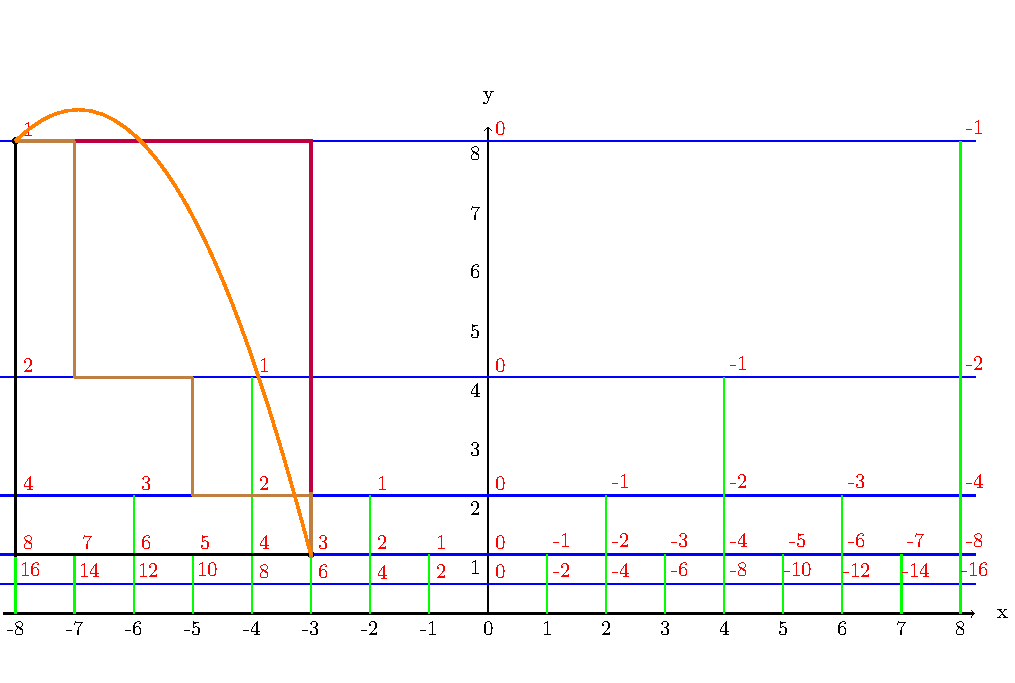
\includegraphics{images/06-example-canonical-form}}
\caption{different encodings and their canonical form}\label{fig:canonicalform}
\end{figure}

All of the paths in Figure~\ref{fig:canonicalform} have the same source $1$ and same target $3$.
We will discuss a canonical form for these paths.

It is easy to see that the expressions can be transformed into each other by using the multiplication distributive law and by combining and decomposing terms.

Conversion form brown path to black path
\begin{align}
3 & = ((((((1 - \frac{1}{8}) \times 2) - \frac{1}{2}) \times 2) - 1) \times 2) \\
& = 1 \times 8 -  \frac{1}{8} \times 8 - \frac{1}{2} \times 4 - 1 \times 2 \\
& = ((1 \times 8) - 5)
\end{align}

Conversion form brown path to purple path
\begin{align}
3 & = ((((((1 - \frac{1}{8}) \times 2) - \frac{1}{2}) \times 2) - 1) \times 2) \\
& = (1 - \frac{1}{8}) \times 8 - \frac{1}{2} \times 4 - 1 \times 2 \\
& = (1 - \frac{1}{8}) \times 8 - \frac{1}{4} \times 8 -  \frac{1}{4} \times 8 \\
& = (1 - \frac{1}{8} - \frac{1}{4} - \frac{1}{4}) \times 8 \\
& = ((1 - \frac{5}{8}) \times 8)
\end{align}

Therefore, we can define the black and purple paths in Figure~\ref{fig:canonicalform} as a pair of canonical paths,
which represent all threadlike expressions connecting the source $1$ and the target $3$.

Once we have such canonical paths, we can determine the canonical form of the whole space relative to an arbitrary source point $O$ and any other target point $P$.
This allows us to define the space as a space of threadlike expressions.
\subsection{Currying and path notation}\label{subsec:currying}

Currying is a basic technique in functional programming\cite{Reynolds1972DefinitionalIF},
which is used to transform a function with multiple arguments into a sequence of functions with one argument.
By currying a threadlike arithmetic expression, we can obtain a sequence of functions that operate on an operand, which is the leftmost leaf node.

We introduce the following notation for currying a threadlike arithmetic expression:
\begin{itemize}
    \item initial operand: the leftmost leaf node
    \item operator: $\oplus_y: x \mapsto x + y$
    \item operator: $\ominus_y: x \mapsto x - y$
    \item operator: $\otimes_y: x \mapsto x \cdot e^y$
    \item operator: $\oslash_y: x \mapsto x \cdot e^{-y}$
\end{itemize}

For example, the threadlike arithmetic expression $(((((1 \times 2) \times 2) + 1) \times 3) + 6)$ can be curried as

\[\oplus_6(\otimes_{\ln 3}(\oplus_1(\otimes_{\ln 2}(\otimes_{\ln 2}(1)))))\]

Suppose we have a series of operators $a_1, a_2, \cdots a_{n-1}, a_n$, we introduce a \emph{path notation}.

\[x a_1 a_2 \cdots a_{n-1} a_n \coloneqq a\_n( a_{n-1}( \cdots a_2( a_1(x) ) \cdots ) )\]

So, the above example can be written as

\[1 \otimes_{\ln 2} \otimes_{\ln 2} \oplus_1 \otimes_{\ln 3} \oplus_6 \]

If a path begins with a number, we refer to it as a \emph{bounded path}.
If it does not, we refer to it as a \emph{free path}, similar to the concept of vectors from the origin versus vectors at arbitrary points.
a bounded path results in a number, while a free path results in a function.

Now we will verify that the operators within a path are associative.

\begin{lemma}\label{lemma:associative}
    The operators within a path are associative, i.e. we have \[a [b c] = [a b] c\]
\end{lemma}

\begin{proof}
We use normal typeface to express the path notation, and bold typeface to express the function notation.

For a free path, follow the definition, we have
\[a [b c] = [b c](\mathbf{a}) = \mathbf{c}(\mathbf{b}(\mathbf{a}))\]
\[[a b] c = \mathbf{c}([a b]) = \mathbf{c}(\mathbf{b}(\mathbf{a}))\]

hence, we have
\[a [b c] = [a b] c\]
is hold for a free path.

For a bounded path, we have
\[x a [b c] = [b c](\mathbf{a}(x)) = \mathbf{c}(\mathbf{b}(\mathbf{a}(x)))\]
\[x [a b] c = \mathbf{c}([a b](x)) = \mathbf{c}(\mathbf{b}(\mathbf{a}(x)))\]

hence, we have
\[a [b c] = [a b] c\]
is hold for a bounded path.

\end{proof}

\begin{definition}\label{definition:concatenate}
    The concatenation of paths $p_1 \cdot p_2$ is defined as the composite of functions:
    \[p_1 \cdot p_2 \coloneqq p_2 \circ p_1 \]
\end{definition}

When a sequence of paths is concatenated, and only the first path can be bounded.
If the first path is bounded, the concatenated result is a bounded path.
Otherwise, the concatenated result is a free path.

\subsection{Alternating threadlike expressions}\label{subsec:alternating}

Now we can define alternating threadlike expressions, which were mentioned in Section~\ref{sec:expression}, using the path notion.

\begin{equation}\label{eq:alternative}
    \alpha = a_1 b_1 a_2 b_2 \cdots a_l b_l, a_i = \otimes_{\lambda_i}, b_i = \oplus_{\mu_i}, \lambda_i, \mu_i \in \mathbb{R}
\end{equation}

where $\bigoplus$ and $\bigotimes$ denote addition and multiplication, respectively,
and the expression is a zigzag of alternating addition and multiplication operations.
$\alpha$ is a free path, and we can bind a number to it.

Since $0$ is the identity element for addition and $1$ is the identity element for multiplication,
it is straightforward to see that any arithmetic expression can be converted into an alternating threadlike expression
by introducing more $0$ and $1$ into the original expression.
So alternating threadlike expression is a kind of canonical form.

We can derive a formula for perturbations in alternating threadlike expressions.

Let us define the left-to-right accumulated sum of $\lambda_i$ as $\check{\lambda}_i$, such that:
\begin{equation}
\check{\lambda}_i = \sum_{j=1}^i \lambda_j, \check{\lambda}_0 = 0\label{eq:accsumlr}
\end{equation}

Then we also have right-to-left accumulated sum of $\lambda_i$
\begin{equation}
\hat{\lambda}_i = \check{\lambda}_l - \check{\lambda}_{l - i}, \hat{\lambda}_0 = 0\label{eq:accsumrl}
\end{equation}

Expanding equation~\eqref{eq:alternative} using the distributive law and the above notion at point $\mu_0$, we obtain:
\begin{align}
\alpha(\mu_0) & = e^{\lambda_l}(\cdots (e^{\lambda_2} (e^{\lambda_1} \mu_0 + \mu_1) + \mu_2) \cdots) + \mu_l \\
& = e^{\hat{\lambda}_l} \mu_0 + e^{\hat{\lambda}_{l - 1}} \mu_1  + e^{\hat{\lambda}_{l - 2}} \mu_2 + \cdots + e^{\hat{\lambda}_1} \mu_{l - 1} + e^{\hat{\lambda}_0} \mu_l
\end{align}

Next, at the starting point $\mu_0$, we introduce a perturbation $\tilde{\mu}_0 = e^{\eta_0} \mu_0 + \epsilon_0$,
where $\eta_0$ and $\epsilon_0$ are the disturbance terms added by the summation and multiplication operations, respectively. Then, we have:
\begin{align}
\alpha(\tilde{\mu}_0) & = e^{\hat{\lambda}_l} (\tilde{\mu}_0) + e^{\hat{\lambda}_{l - 1}} \mu_1  + e^{\hat{\lambda}_{l - 2}} \mu_2 + \cdots + e^{\hat{\lambda}_1} \mu_{l - 1} + e^{\hat{\lambda}_0} \mu_l \\
& = \alpha(\mu_0) + e^{\hat{\lambda}_l} (\tilde{\mu}_0 - \mu_0)
\end{align}

As a result, purely from an arithmetic perspective, without the need for limits, we can derive the following meaningful ratio:
\begin{equation}
\frac{\alpha(\tilde{\mu}_0) - \alpha(\mu_0)}{\tilde{\mu}_0 - \mu_0} = e^{\hat{\lambda}_l} = e^{\check{\lambda}_l}\label{eq:ratio}
\end{equation}

Now we extend this relationship from the starting point $\mu_0$ to the entire process, we define the recursive formula

\[
w_i = e^{\lambda_i} w_{i-1} + \mu_i, w_0 = 0
\]

and then we have

\begin{equation}
\frac{\tilde{w}_i - w_i}{\tilde{\mu}_0 - \mu_0} = e^{\check{\lambda}_i}, i \in \{1, ..., l\}\label{eq:perturbation1}
\end{equation}

So, we have

\[
\tilde{w}_i - w_i = e^{\check{\lambda}_i} (\tilde{\mu}_0 - \mu_0)
\]

and hence

\begin{equation}
\tilde{w}_i - w_i = e^{\lambda_i}(\tilde{w}_{i - 1} - w_{i - 1})\label{eq:perturbation2}
\end{equation}

That means the perturbation along the path is controlled by the multiplication terms of $e^{\lambda_i}$.

\subsection{Generated structure, commutator and arithmetic torsion}\label{subsec:generated-structure}

In order to study mesh grids like the one described in subsection~\ref{subsec:meshgrid},
we need to investigate the algebraic structure of the threadlike arithmetic expressions that are generated.

For real number $\mathbb{R}$ and elements $\mu, \lambda \in \mathbb{R}$, we consider all the arithmetical expressions
that are freely generated from
\begin{itemize}
    \item initial operand: $0$
    \item operator: $\oplus_\mu: x \mapsto x + \mu$
    \item operator: $\ominus_\mu: x \mapsto x - \mu$
    \item operator: $\otimes_\lambda: x \mapsto x \cdot e^\lambda$
    \item operator: $\oslash_\lambda: x \mapsto x \cdot e^{- \lambda}$
\end{itemize}

We denote these expressions as $E(\mu, \lambda)$, where $\mu$ is the additional generator and $e^\lambda$ is the multiplicative generator.
In cases where the context is clear, we may omit $\mu$ and $\lambda$ from the index.
Our goal is not to study only a single $E(\mu, \lambda)$, but rather to use a family of $E(\mu, \lambda)$ to approach a continuous space.

Since $\oplus_\mu$ and $\ominus_\mu$ are mutually inverse operations, it follows that $\otimes_\lambda$ and $\oslash_\lambda$ are also mutually inverse. This means that $E(\mu, \lambda)$ forms a group.
An intriguing observation is that the commutator of this group is not equal to identity generally,
especially the commutator of the generators.

\begin{equation}
x \oplus_\mu \otimes_\lambda \ominus_\mu \oslash_\lambda - x = \mu(1 - e^{-\lambda})\label{eq:commutator1}
\end{equation}
\begin{equation}
x \otimes_\lambda \oplus_\mu \oslash_\lambda \ominus_\mu - x = - \mu(1 - e^{-\lambda})\label{eq:commutator2}
\end{equation}

Formula \ref{eq:commutator1} obey the right-hand rule, and formula \ref{eq:commutator2} obey the left-hand rule.

Or equivlently\footnote{Please reference section \ref{subsec:descartes-coordinate}, the equivlence here is refered to the same order of the infinitesimal}, we define below difference $\tau$ obey the right-hand rule:

\begin{equation}
\tau = x \oplus_\mu \otimes_\lambda - x \otimes_\lambda \oplus_\mu = \mu(e^\lambda - 1)\label{eq:torsion}
\end{equation}

These differences are constant, indicating a type of torsion in the generated group.
And torsion $\tau$ is specifically referred to as the arithmetic torsion.

We will reveal that $\tau$ is related to the curvature of the surface in later sections.

\subsection{Problems on equality, singularity, symmetries}\label{subsec:problems-on-equality-singularity-symmetries}

From the perspective of computer science, it is useful to consider different levels of equality within freely generated structures.
\begin{itemize}
\item Literal equality: the finest level of equality, judged by the string representation of the expression
\item Syntactical equality: equality under certain syntactical rules
\begin{itemize}
\item When inverse operators exist, it forms a group
\item When the commutative and distributive laws exist, it can be considered an algebra
\end{itemize}
\item Semantic equality: the coarsest level of equality, judged by the evaluation of the expression
\end{itemize}

Literal equality is the strictest level of equality, and two different threadlike expressions are considered equal only if their string representations are exactly the same.
This level of equality may be too strict, as it may not be compatible with the evaluation of the expression.
However, under literal equality, the generated structure is the most rich and provides the base textures that can be woven into a space.

Semantic equality is the least strict level of equality, and two different threadlike expressions are considered equal if they evaluate to the same number.
This level of equality provides the total symmetrical resources of the space.

We can think of literal equality as the bottom and semantic equality as the top of a lattice,
with syntactical equality being a compromise between the two extremes.

To end this introduction part of the paper, we present several problems and speculations that drives our research.
These important problems arise from distance between syntactical and semantic structures.

\emph{Foundational problem}: A careful reader may have noticed that the definition~\ref{def:arithmetic-expression} is based on rational numbers $\mathbb{Q}$.
Why can't we use real numbers $\mathbb{R}$ instead?
The answer is that syntactically valid expressions may not be semantically valid.
Dividing by zero can lead to invalid expressions, and the evaluation of the expression cannot be defined in this situation.
Therefore, in real numbers, an expression may be syntactically valid but semantically not valid,
and there is no algorithm that can decide whether an expression is semantically valid or not.
How can we bridge this gap and provide a continuous geometry space?
We will attempt to partially solve this problem in some special cases in section~\ref{sec:topology}.

\emph{Singular point problem}: We have a very strong intuition that semantically invalid expressions lead to singular points.
The way we discussed in complex analysis may be borrowed here: essential singularities and poles.

\emph{Symmetry and classification problem}: We conjecture that the equality lattice may not only play a role in the construction of a space, but also determine the symmetry of that space.
We can imagine that, at certain levels of the lattice, we weave syntactically generated substructures into points to form a space,
and the weaving process uses up some symmetrical resources, leaving the rest to form a symmetry on the space.
The structure within the total symmetry may provide us with a systematic way of constructing spaces, and allow us to classify spaces based on their symmetries.

\newpage

\section{Flow equation}\label{sec:flowequation}

\subsection{Flow equation}\label{sec:equation}

Consider an infinitesimal generating process on a Riemannian surface $M$ using two generators:
one for an additional action $\mu$ and the other for a multiplicative action $e^\lambda$.
These two generators are perpendicular.
This generation process produces an assignment $A: M \to R$ over the surface.

For any point with an assignment $a_0$, if we consider a movement of distance $\epsilon$ in a direction with angle $\theta$
over a time period of $\delta$, we can establish the following:

\[
    a_{\delta} = (a_0 + \mu \epsilon \cos \theta)e^{\lambda \epsilon \sin \theta}
\]

or

\[
    a_{\delta} = a_0 e^{\lambda \epsilon \sin \theta} + \mu \epsilon \cos \theta
\]

Both formula can be simplified to the same result:

\[
    a_{\delta} = a_0 + \epsilon (a_0 \lambda \sin \theta + \mu \cos \theta)
\]

Then, we have the following equation:

\[
    \frac{1}{\delta} (a_{\delta} - a_0) = \frac{\epsilon}{\delta} (\mu \cos \theta + x_0 \lambda \sin \theta)
\]

When both $\delta$ and $\epsilon$ are towards zero, we get $da / dt$, and hence

\[
    \frac{da}{dt} = u (\mu \cos \theta + a \lambda \sin \theta)
\]

Or, we can change it to another form

\begin{equation}
    \frac{da}{ds} = \mu \cos \theta + a \lambda \sin \theta\label{eq:flow}
\end{equation}

We name this equation~\eqref{eq:flow} as the flow equation.

The left side of this equation is governed by the distance structure, while the right side is governed by the angle structure.
This leads to below theorem.

\begin{theorem}
Isometries keep the flow equation\eqref{eq:flow}
\label{thm:isometry}
\end{theorem}

\begin{proof}
  An isometry keeps both the distance structure and the angle structure, so it keeps the flow equation.
\end{proof}

We can also get a direct formal solution of the flow equation~\eqref{eq:flow}(details in Appendix~\ref{sec:directformalsolution}).

\begin{equation}
   a = (a_0 + \frac{\mu}{\lambda} \cot \theta) e^{\lambda s \sin \theta} - \frac{\mu}{\lambda} \cot \theta\label{eq:solution}
\end{equation}

While the validity of this solution is still uncertain because we have not assumed any constraints on the local coordinate system,
it is still a useful starting point for further investigation.
For example, we can use this solution to derive (details in Appendix~\ref{sec:conformance}) the relationship between assignments at different vertices in a cell of a mesh grid.

Assuming the assignment at the center point of a cell is $a_0$, we move in different directions and obtain the following assignments:

\begin{itemize}
\item $\theta = 0$: $a_s = a_0 + \mu s$
\item $\theta = \frac{\pi}{2}$: $a_s = a_0 e^{\lambda s}$
\item $\theta = \pi$: $a_s = a_0 - \mu s$
\item $\theta = \frac{3 \pi}{2}$: $a_s = a_0 e^{- \lambda s} $
\end{itemize}

This result is straightforward, but it demonstrates that the infinitesimal generating process is consistent with the discrete mesh grid.

\subsection{The contour-gradient form of flow equation}\label{subsec:the-contour-gradient-form}

It is easy to derive the contour equation in the local coordinate

\begin{equation}
    \mu \cos \theta_c + a \lambda \sin \theta_c = 0\label{eq:contour}
\end{equation}

then we have

\begin{equation}
    \theta_c = - \arctan \frac{\mu}{a \lambda}\label{eq:contourangle}
\end{equation}

the contour and the gradient are perpendicular to each other

\begin{equation}
    \theta_g = \pm \frac{\pi}{2} - \arctan \frac{\mu}{a \lambda}\label{eq:gradientangle}
\end{equation}

then along $\theta_g$ we have

\begin{equation}
    \frac{da}{ds} = \mu \cos (\pm \frac{\pi}{2} - \arctan \frac{\mu}{a \lambda}) + a \lambda \sin (\pm \frac{\pi}{2} - \arctan \frac{\mu}{a \lambda})
    \label{eq:alonggradient}
\end{equation}

\begin{equation}
    \frac{da}{ds} = \pm \sqrt{\mu^2 + \lambda^2 a^2}\label{eq:grad}
\end{equation}

By introducing the right-hand rotation angle $\phi$ along the gradient direction, we can establish a local polar coordinate system based on the gradient and contour lines.
Then the growth rate of $a$ along the angle $\phi$ is

\begin{equation}
    \frac{da}{ds} = \mu \cos (\frac{\pi}{2} - \arctan \frac{\mu}{a \lambda} + \phi) + a \lambda \sin (\frac{\pi}{2} - \arctan \frac{\mu}{a \lambda} + \phi)
    \label{eq:fourfold}
\end{equation}

And the simplified equation is

\begin{equation}
    \frac{da}{ds} = \sqrt {\mu^2 + a^2 \lambda^2} \cos \phi\label{eq:contourgradient}
\end{equation}

The equation~\eqref{eq:contourgradient} is the flow equation in the contour-gradient coordinate system.

Equation~\eqref{eq:contourgradient} is solvable, and we get the relation between $a$ and $s$:

\begin{equation}\label{eq:rel_a_s}
    \tanh(\lambda s \cos \phi - c) = \frac{\lambda a}{\sqrt{\mu^2 + \lambda^2 a^2}}
\end{equation}

we can further simplify the equation to

\begin{equation}
  a = \pm \frac{\mu}{\lambda} \sinh(\lambda s \cos \phi - c)\label{eq:gradevo}
\end{equation}

Under the initial condition $a = a_0$ when $s = 0$, we can get the following equation:

\begin{equation}
    a = \frac{\mu}{\lambda} \sinh(\lambda s \cos \phi + \arcsinh \frac{a_0 \lambda}{\mu})\label{eq:gradevo2}
\end{equation}

or

\begin{equation}
    a = - \frac{\mu}{\lambda} \sinh(\lambda s \cos \phi - \arcsinh \frac{a_0 \lambda}{\mu})\label{eq:gradevo3}
\end{equation}

In this coordinate system, the additional line and the multiplicative line are:

\begin{equation}
    \phi = \arccos \frac{\mu}{\sqrt {\mu^2 + a^2 \lambda^2}} \label{eq:additionalline}
\end{equation}

\begin{equation}
    \phi = \arcsin \frac{\mu}{\sqrt {\mu^2 + a^2 \lambda^2}}\label {eq:mulitiplcativeline}
\end{equation}

\subsection{Flow and function}\label{subsec:flow-and-function}

In this section, we aim to present novel insight into functions.
Namely, the treatment of functions as flows will be discussed.

\begin{definition}\label{def:projection}
Given a function $k$ on the real domain $R$, we can introduce a mapping $l$ on the arithmetic expression space $H$ such that the following diagram commutes.

\begin{center}
    \begin{tikzcd}
        H && H \\
        R && R
        \arrow["l", from=1-1, to=1-3]
        \arrow["\nu"', from=1-1, to=2-1]
        \arrow["\nu", from=1-3, to=2-3]
        \arrow["k"', from=2-1, to=2-3]
    \end{tikzcd}
\end{center}

where $\nu$ is the evaluation function of the expression. Then we call the mapping $l$ is the promotion of the function $k$,
or function $k$ is the projection of the mapping $l$.
\end{definition}

A mapping $l$ on the arithmetic expression space $H$ can be implemented by a geometry flow on $M$.
We give an example of function $\sin$ as follows.

\subsection{The existence theorems}\label{subsec:existence-theorems}

There are two important existence theorems related to the flow equation~\eqref{eq:flow}.

The first existence theorem states that if we have a Riemann surface $M$, then there exists a function $a$ on $M$ that satisfies the flow equation~\eqref{eq:flow}. This theorem is proved in a later section, and we will not go into the details of the proof here.

\begin{theorem}
    Given a Riemann surface $M$, there exists a function $a$ on $M$ satisfying the flow equation~\eqref{eq:flow}.
    \label{prop:existence1st}
\end{theorem}

The second existence theorem is also crucial.
It says that if we have a smooth surface $S$ and a function $a$ on $S$, then we can find a metric $g$ on $S$ that makes $a$ satisfy the flow equation~\eqref{eq:flow}.

\begin{theorem}(By Le Zhang)
    Given an oriented Riemannian surface $S$, and a function $a$ over $S$, there exists a metric $g$ on $S$ that makes $a$
    satisfying the flow equation~\eqref{eq:flow}.
    \label{prop:existence2nd}
\end{theorem}

\begin{proof}
    The proof consists of two main steps. First, we demonstrate the existence of a metric \( g \) on \( S \) that allows \( a \) to satisfy the flow equation~\eqref{eq:flow} in a local coordinate system. Then, we show that this local metric can be extended to a global metric on \( S \).

    \emph{Part 1: Local Perspective}

    Consider a point \( p \) on the surface \( S \), and there is a neighborhood \( U \) around \( p \).
    In this area, we can find a local isothermal coordinate system in which the metric takes the form:
    \[ ds^2 = e^{2\rho}(du^2 + dv^2), \]
    where \( u \) and \( v \) are the coordinates of \( U \), and \( \rho \) is a function of \( u, v \) in \( U \).
    The gradient of \( a \) in this local isothermal coordinate system is expressed as:
    \[ \nabla a = \frac{\partial a}{\partial u} du + \frac{\partial a}{\partial v} dv. \]
    Using the definition of the directional derivative, we obtain:
    \[ \frac{da_{\phi}}{ds_{\phi}} = ||\nabla a|| \cos \phi, \]
    where \( ||\nabla a|| \) is the norm of \( \nabla a \), and \( \phi \) is the angle between \( \nabla a \) and the direction of movement.

    Now, considering the flow equation in the gradient-contour coordinate system, we arrive at:
    \[ \frac{da_{\phi}}{ds_{\phi}} = \sqrt{\mu^2 + a^2 \lambda^2} \cos \phi. \]

    Note that \( ||\nabla a|| \) is fixed for the given function \( a \) and the local coordinate system, and \( \sqrt{\mu^2 + a^2 \lambda^2} \) is also fixed for the given function \( a \). Thus, we can scale \( \rho \) with a linear factor to make \( ||\nabla a|| \) match the fixed value of \( \sqrt{\mu^2 + a^2 \lambda^2} \). Specifically, we can find a morphing ratio \( \kappa \) as follows:

    \begin{align}
    ds^2 &= \kappa e^{2 \rho}(du^2 + dv^2)\label{eq:morphing} \\
         &= \kappa ||\nabla a|| \\
         &= \sqrt{\mu^2 + a^2 \lambda^2},
    \end{align}

    yielding:
    \begin{equation}
        \kappa = \frac{\sqrt{\mu^2 + a^2 \lambda^2}}{||\nabla a||}\label{eq:ratio}
    \end{equation}

    This value of \( \kappa \) allows us to morph the local isothermal coordinate into a gradient-contour coordinate,
    and thus the flow equation~\eqref{eq:flow} can be satisfied in the final local coordinate system.
    The morphing is controlled by the equation~\eqref{eq:morphing}, and the morphing ratio \( \kappa \) is varied from $1$ to the value of~\eqref{eq:ratio}.

    \emph{Part 2: Global Perspective}




    \qedhere
\end{proof}


\newpage

\section{The first kind space $\mathfrak{E}_1$}\label{sec:firstkind}

This section introduces the first kind arithmetic expression space ($\mathfrak{E}_1$), providing a geometric framework for analyzing arithmetic expressions. The space is constructed on the upper half-plane with a hyperbolic metric: $ds^2 = \frac{1}{y^2} (dx^2 + dy^2)$, where the assignment function $a = - \frac{x}{y}$ satisfies the flow equation and serves as an eigenfunction of the Laplacian with eigenvalue 2.

Two equivalent examples of $\mathfrak{E}_1$ are presented: the upper half-plane model and a horocycle-based coordinate system, connected through Möbius transformation. The section explores geometric propagation mechanisms, showing how the assignment value propagates like expanding concentric circles in hyperbolic space. It examines grid structures in $\mathfrak{E}_1$, revealing dual grids reflecting the geometric structure of the Baumslag-Solitar group, and demonstrates how arithmetic torsion corresponds precisely to hyperbolic areas enclosed between evaluation paths. The section concludes by introducing tube structures, which extend $\mathfrak{E}_1$ to parameterized families, enabling analysis of how expressions evolve across parameter variations.

\subsection{Foundational exemplars}\label{subsec:motivexamples}

We present two analytically equivalent examples that belong to the class of spaces designated as the first kind arithmetic expression space $\mathfrak{E}_1$.

\subsubsection{Example 1: Upper Half Plane Model}

Consider the upper half plane ${\mathcal{H}: (x, y) \ | \ y > 0}$ equipped with the following inner product and metric tensor:

$$
\mathbf{a} \cdot \mathbf{b} = \begin{bmatrix} a_x & a_y \end{bmatrix} \begin{bmatrix} \frac{1}{y^2} & 0 \\ 0 & \frac{1}{y^2} \end{bmatrix} \begin{bmatrix} b_x \\ b_y \end{bmatrix}
$$

$$
ds^2 = \frac{1}{y^2} (dx^2 + dy^2)
$$

On this manifold, we define an assignment field $a$ as follows:

\begin{equation}\label{eq:exmp1}
a = - \frac{x}{y}
\end{equation}

\begin{theorem}\label{thm:exmp1}
The assignment $a$ defined by formula \eqref{eq:exmp1} satisfies the flow equation \eqref{eq:flow}.
\end{theorem}

\begin{proof}
We initiate with the differential of the assignment:
$$
da = d\left(-\frac{x}{y}\right) = \frac{xdy - ydx}{y^2} = -\frac{dx + ady}{y}
$$

The differential of arc length is given by:
$$
ds = \frac{\sqrt{dx^2 + dy^2}}{y}
$$

Therefore:
$$
\frac{da}{ds} = - \frac{dx + ady}{y} \cdot \frac{y}{\sqrt{dx^2 + dy^2}} = - \frac{dx + ady}{\sqrt{dx^2 + dy^2}}
$$

In the local coordinate system determined by $(-1, 0)$ and $(0, -1)$ under the right-hand rule, we have:
$$
\cos \theta = \frac{-dx}{\sqrt{dx^2 + dy^2}} \quad \text{and} \quad \sin \theta = \frac{-dy}{\sqrt{dx^2 + dy^2}}
$$

Substituting these values:
$$
\frac{da}{ds} = \cos \theta + a \sin \theta
$$

This precisely corresponds to the flow equation \eqref{eq:flow} with $\mu=1$ and $\lambda=1$.
\end{proof}

We can verify that $a$ constitutes an eigenfunction of the Laplacian operator:
$$
\Delta a = - y^2 \left(\frac{\partial^2 a}{\partial x^2} + \frac{\partial^2 a}{\partial y^2}\right) = y^2 \left(\frac{\partial}{\partial y} \left(\frac{\partial}{\partial y} \frac{x}{y}\right)\right) = 2a
$$

\subsubsection{Example 2: Horocycle-Based Coordinate System}

For our second exemplar, we introduce a horocycle-based coordinate system for hyperbolic surfaces. This global coordinate system comprises two orthogonal families of curves: horocycles sharing the same ideal point, and geodesics perpendicular to these horocycles.

\begin{figure}[ht]
\centering
\resizebox{0.5\textwidth}{!}{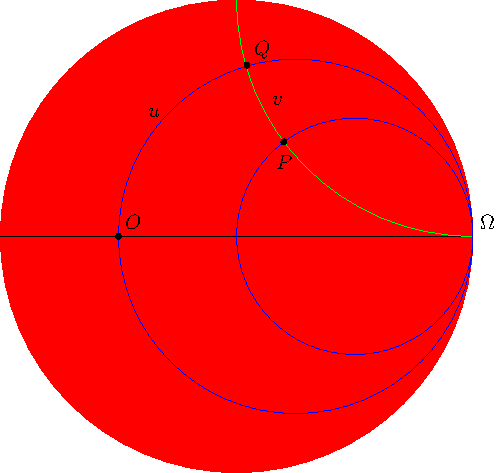
\includegraphics{images/11-horocyclebased}}
\caption{A horocycle-based coordinate system on the Poincaré disc. Blue curves represent horocycles tangent at ideal point $\Omega$, green lines depict perpendicular geodesics.}\label{fig:horocyclecoord}
\end{figure}

On the Poincaré disc $\mathcal{P}$, the coordinates of a point $P$ are denoted by $(u,v)$, where:
\begin{itemize}
\item $u$ represents the signed length of $OQ$
\item $v$ represents the signed length of $QP$
\item The sign conventions adhere to the right-hand rule and orientation relative to the ideal point $\Omega$
\end{itemize}

We equip this coordinate system with the inner product:
$$
\mathbf{a} \cdot \mathbf{b} = \begin{bmatrix} a_u & a_v \end{bmatrix} \begin{bmatrix} e^{-2v} & 0 \\ 0 & 1 \end{bmatrix} \begin{bmatrix} b_u \\ b_v \end{bmatrix}
$$

And the corresponding metric tensor:
$$
ds^2 = e^{-2v} du^2 + dv^2
$$

The Laplacian operator in this coordinate system is expressed as:
$$
\Delta = e^{2v} \frac{\partial^2}{{\partial u}^2} + \frac{\partial^2}{{\partial v}^2} - \frac{\partial}{\partial v}
$$

In this coordinate framework, we define an assignment:

\begin{equation}\label{eq:exmp2}
a = u e^{-v}
\end{equation}

\begin{theorem}\label{thm:exmp2}
The assignment $a$ defined by formula \eqref{eq:exmp2} satisfies the flow equation \eqref{eq:flow}.
\end{theorem}

\begin{proof}
We establish this result by demonstrating that examples 1 and 2 are equivalent through a Möbius transformation. Consider the complex representation of the upper half plane:
$$
z = x + yi
$$

The Möbius transformation mapping the upper half plane to the Poincaré disc is given by:
$$
z \mapsto \frac{z-i}{z+i}
$$

\begin{figure}[ht]
\centering
\resizebox{0.8\textwidth}{!}{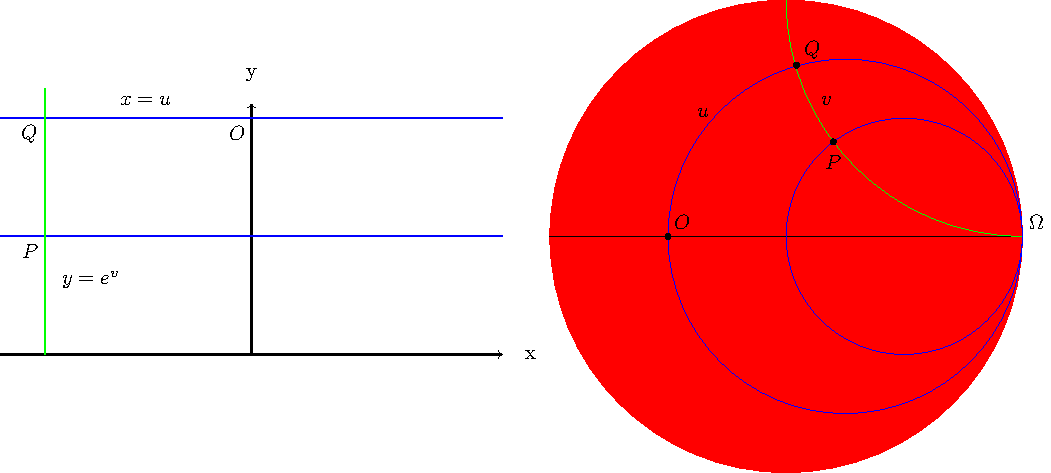
\includegraphics{images/12-proofbymapping}}
\caption{Mapping between the upper half plane and Poincaré disc models}\label{fig:mapping}
\end{figure}

This conformal transformation maps horizontal lines in $\mathcal{H}$ to horocycles sharing the ideal point $\Omega = 1$ in $\mathcal{P}$, and vertical geodesics in $\mathcal{H}$ to perpendicular geodesics in $\mathcal{P}$.

Expressed in the target coordinate system, this transformation yields:
$$
\begin{cases}
x = u\\
y = e^v \\
\end{cases}
$$

Substituting into the assignment from Example 1:
$$
a = -\frac{x}{y} = -\frac{u}{e^v} = -u e^{-v}
$$

Since the Möbius transformation is conformal and preserves the flow equation, and accounting for the orientation change, we obtain $a = u e^{-v}$ satisfying the flow equation.
\end{proof}

As in Example 1, we can verify that $a$ constitutes an eigenfunction of the Laplacian:
$$
\Delta a = e^{2v} \frac{\partial^2(u e^{-v})}{{\partial u}^2} + \frac{\partial^2(u e^{-v})}{{\partial v}^2} - \frac{\partial(u e^{-v})}{\partial v} = 2a
$$

These two examples, emerging from the same geometric foundation but expressed in different coordinate systems, demonstrate the fundamental properties of the first kind arithmetic expression space.

\subsection{Theoretical framework of $\mathfrak{E}_1$ space}\label{subsec:generalframework}

Building upon the foundational exemplars, we now establish a comprehensive theoretical framework for the first kind arithmetic expression space $\mathfrak{E}_1$. 

Consider the upper half plane $\mathcal{B}$:
$$
\{\mathcal{B}: (x, y) | y > 0 \}
$$

equipped with an inner product and metric tensor parameterized by constants $\mu$ and $\lambda$:

$$
\mathbf{a} \cdot \mathbf{b} = \begin{bmatrix} a_x & a_y \end{bmatrix} \begin{bmatrix} \frac{1}{\mu^2 y^2} & 0 \\ 0 & \frac{1}{\lambda^2 y^2} \end{bmatrix} \begin{bmatrix} b_x \\ b_y \end{bmatrix}
$$

$$
ds^2 = \frac{1}{y^2}\left(\frac{dx^2}{\mu^2} + \frac{dy^2}{\lambda^2}\right)
$$

The assignment function in this generalized framework maintains the form:

\begin{equation}\label{eq:genassignment}
a = - \frac{x}{y}
\end{equation}

This defines the first kind arithmetic expression space $\mathfrak{E}_1$, characterized by the following theorem:

\begin{theorem}\label{thm:generalE1}
The assignment $a$ given by \eqref{eq:genassignment} satisfies the flow equation \eqref{eq:flow} with parameters $\mu$ and $\lambda$, independent of the specific values of these generators.
\end{theorem}

\begin{proof}
The differential of the assignment is given by:
$$
da = d\left(-\frac{x}{y}\right) = \frac{xdy - ydx}{y^2} = -\frac{dx + a dy}{y}
$$

The differential of arc length is expressed as:
$$
ds = \frac{1}{y}\sqrt{\frac{dx^2}{\mu^2} + \frac{dy^2}{\lambda^2}}
$$

Therefore:
$$
\frac{da}{ds} = - \frac{dx + a dy}{y} \cdot \frac{y}{\sqrt{\frac{dx^2}{\mu^2} + \frac{dy^2}{\lambda^2}}} = -\frac{dx + a dy}{\sqrt{\frac{dx^2}{\mu^2} + \frac{dy^2}{\lambda^2}}}
$$

In the local coordinate system determined by $(-1, 0)$ and $(0, -1)$ according to the right-hand rule:

$$
\cos \theta = \frac{-\frac{dx}{\mu}}{\sqrt{\frac{dx^2}{\mu^2} + \frac{dy^2}{\lambda^2}}} \quad \text{and} \quad \sin \theta = \frac{-\frac{dy}{\lambda}}{\sqrt{\frac{dx^2}{\mu^2} + \frac{dy^2}{\lambda^2}}}
$$

Substituting these values:
$$
\frac{da}{ds} = \mu \cos \theta + a \lambda \sin \theta
$$

This precisely corresponds to the flow equation \eqref{eq:flow} with the given parameters $\mu$ and $\lambda$.
\end{proof}

The $\mathfrak{E}_1$ space is distinguished by its intrinsic connection to hyperbolic geometry and the property that the assignment function $a = -x/y$ constitutes an eigenfunction of the Laplacian operator with eigenvalue 2. This space provides a natural geometric framework for analyzing arithmetic expressions, particularly those involving addition and multiplication operations.

\subsection{Geometric propagation mechanisms}\label{subsec:geompropagation}

The flow equation in the $\mathfrak{E}_1$ space can be interpreted as describing the propagation of arithmetic expressions. This interpretation extends the propagation method discussed in Section \ref{subsec:propagation-method}.

In the $\mathfrak{E}_1$ space, paths along constant $x$ (vertical geodesics in the upper half plane) correspond to multiplication operations, while paths along constant $y$ (horizontal geodesics) correspond to addition operations. The assignment value $a = -x/y$ propagates according to the flow equation as we traverse these paths.

The propagation can be visualized as wavefronts emanating from source points in the upper half plane. Points with identical assignment values form equipotential curves, and the flow equation governs the geometric evolution of these wavefronts.

From equation \eqref{eq:gradevo5}, we recall that along the gradient direction ($\phi=0$) starting from $a_0=0$:
\begin{equation}
a = \pm \frac{\mu}{\lambda} \sinh(\lambda s)
\end{equation}

This expression exhibits a structural similarity to the formula for the circumference of a circle in hyperbolic space with curvature $-\lambda^2$:
\begin{equation}
C = \frac{2\pi}{\lambda} \sinh(\lambda s)
\end{equation}

This correspondence suggests that the assignment $a$ propagates analogously to expanding concentric circles in hyperbolic space, with the zero assignment locus serving as the collection of centroids from which these circles emanate.

The dual perspective of propagation and evaluation provides a powerful framework for understanding arithmetic expressions geometrically:
1. Evaluation of an expression follows geodesic paths through the $\mathfrak{E}_1$ space
2. Different evaluation orders correspond to distinct paths with identical endpoints
3. The flow equation ensures that the final value remains invariant with respect to the path taken (for evaluable expressions)

\subsection{Grid structures}\label{subsec:grids}

A significant geometric characteristic of the first kind arithmetic expression space is the presence of two distinct yet interrelated grid structures, each encoding addition and multiplication operations in different ways. These dual grids reflect the geometric structure of the Baumslag–Solitar group, whose Cayley graph exhibits an anisotropic, hierarchical lattice with a natural correspondence to mixed additive-multiplicative expressions.

Both grid structures are constructed within the upper half-plane model. The first grid is rectilinear, consisting of horizontal lines encoding addition operations and vertical lines encoding multiplication operations. Specifically, this grid is constructed through iterative applications of these two operations to generate a lattice in the $(x,y)$ coordinates. Each horizontal displacement from $(x,y)$ to $(x+1,y)$ represents an addition, and each vertical displacement from $(x,y)$ to $(x,2y)$ represents a multiplication by 2. The grid vertices correspond to values of expressions constructed from repeated applications of addition and multiplication operations, typically originating from a rational base point, often designated as 1.

\begin{figure}[ht]
\centering
\resizebox{0.8\textwidth}{!}{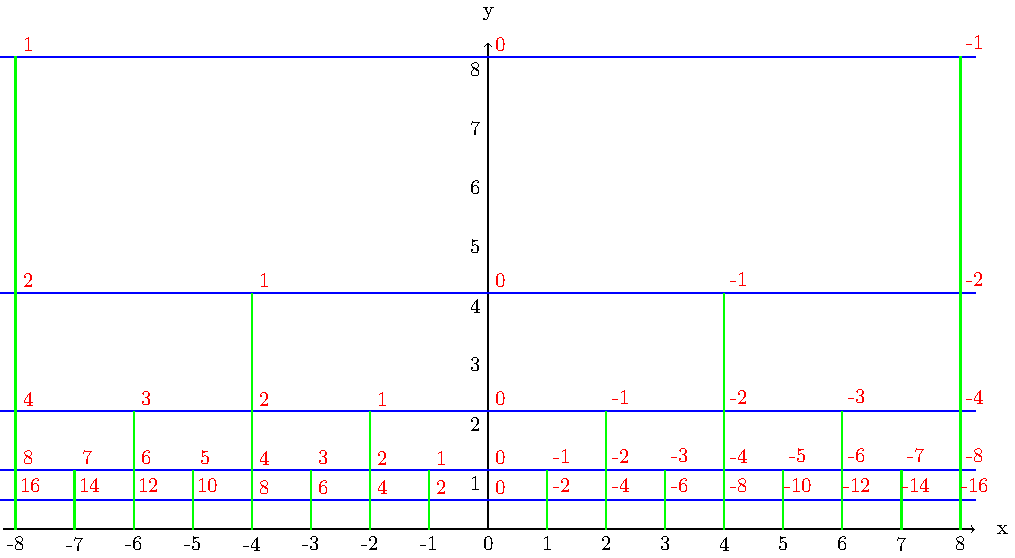
\includegraphics{images/01-grid-example-1}}
\caption{Rectilinear grid structure in the first kind arithmetic expression space $\mathfrak{E}_1$}\label{fig:grid1}
\end{figure}

Notably, in this first grid, the scalar field $a$ remains invariant under variations of the metric parameters $\mu$ and $\lambda$. That is, while the geometric properties of the space (lengths and angles) vary with these parameters, the locus where $a=0$—specifically, the vertical line $x=0$—remains structurally invariant and unaffected by changes in $\mu$ and $\lambda$.

The second grid emerges through a conformal transformation, specifically the Möbius transformation acting within the upper half-plane. This transformation maps horizontal lines to semicircles centered on the real axis and vertical rays to orthogonal semicircles. Under this transformation, the roles of addition and multiplication are effectively interchanged. The addition-multiplication structure of the first grid transforms into a new system of curved geodesics: the images of addition steps now follow curved trajectories around the origin, while the multiplicative steps exhibit contraction and inversion properties.

\begin{figure}[ht]
\centering
\resizebox{0.8\textwidth}{!}{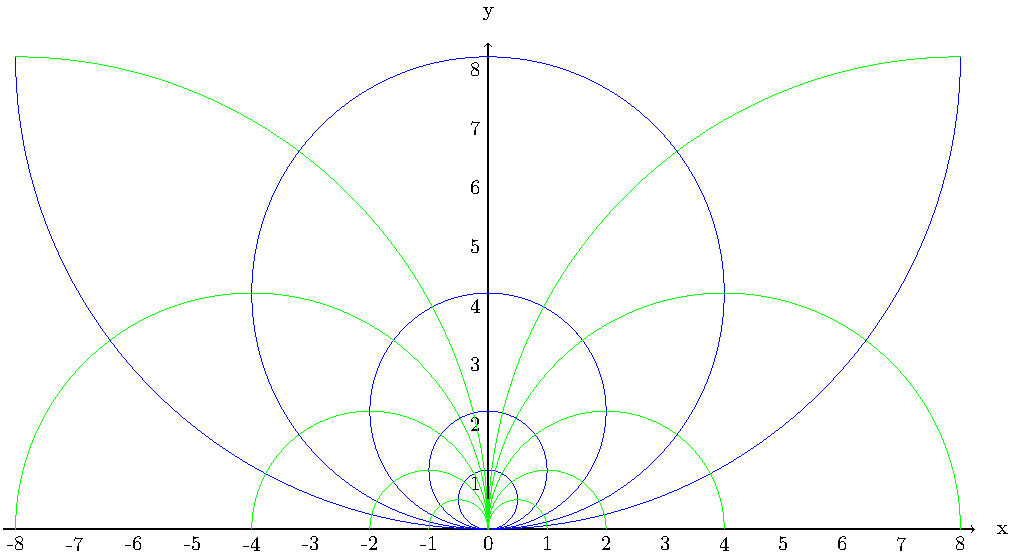
\includegraphics{images/18-grid-example-2}}
\caption{Transformed grid structure in the first kind arithmetic expression space $\mathfrak{E}_1$}\label{fig:grid2}
\end{figure}

Although the visual structure of the second grid exhibits greater complexity, it retains a profound arithmetic coherence. The grid vertices continue to correspond to expressions generated through repeated applications of addition and multiplication operations, albeit composed under the transformed geometry. This grid demonstrates enhanced flexibility: under the conformal transformation, the images of zero lines such as $x=0$ are no longer fixed but deform into dynamic arcs. Consequently, the second grid accommodates a richer family of zero structures, allowing for the possibility of curved, branching, or nested nodal sets that vary with $\mu$, $\lambda$, or the choice of conformal framing.

Each of these grid structures can be interpreted as a geometric realization of a Cayley graph:

\begin{itemize}
\item The rectilinear grid corresponds to the Cayley graph of the Baumslag–Solitar group $BS(1,2)$, where multiplication by 2 followed by addition by 1 follows the relation $b^{-1}ab = a^2$.
\item The transformed (dual) grid corresponds to the Cayley graph of the dual Baumslag–Solitar group, where the roles of addition and multiplication are inverted.
\end{itemize}

Thus, the two grid systems exhibit duality not only in geometric terms but also in group-theoretic structure. The Möbius transformation, acting within the upper half-plane, connects these dual groups by exchanging generators and inverting flow directions, reflecting an intrinsic duality in the geometric composition of arithmetic operations.

The coexistence of these dual grid structures—one linear, one curved—linked via conformal symmetry, suggests a profound underlying symmetry in the geometry of arithmetic expressions. This duality reflects how different evaluation paths or expression embeddings can be interpreted as projections from a common, more complex geometric source. Understanding this symmetry may provide a pathway to expressing arithmetic relations via modular or automorphic structures, particularly in the context of recursive expressions and iterative identities, where Baumslag–Solitar-like behavior naturally emerges.

We conjecture that this grid duality corresponds to a deeper expression-theoretic equivalence, and that the Möbius transformation connecting them manifests an underlying arithmetic symmetry in expression geometry.

\subsection{Torsion under scale transformation}\label{subsec:gridsandtorsion}

The addition-multiplication grid introduced in Section~\ref{subsec:meshgrid} has a natural embedding in the arithmetic expression space $\mathfrak{E}_1$. This grid consists of two orthogonal families of curves:

\begin{enumerate}
    \item \textbf{Addition curves} (blue lines): horizontal geodesics along which $y$ remains constant, representing iterated additions.
    \item \textbf{Multiplication curves} (green lines): vertical or logarithmically scaled geodesics where the ratio $x/y$ remains constant, representing multiplicative transformations.
\end{enumerate}

This grid structure facilitates the geometric analysis of \emph{arithmetic torsion}—a quantity arising from the non-commutativity of certain additive and multiplicative expression sequences. Specifically, torsion quantifies the discrepancy between two seemingly equivalent but differently ordered expressions.

\begin{figure}[ht]
    \centering
    \resizebox{0.8\textwidth}{!}{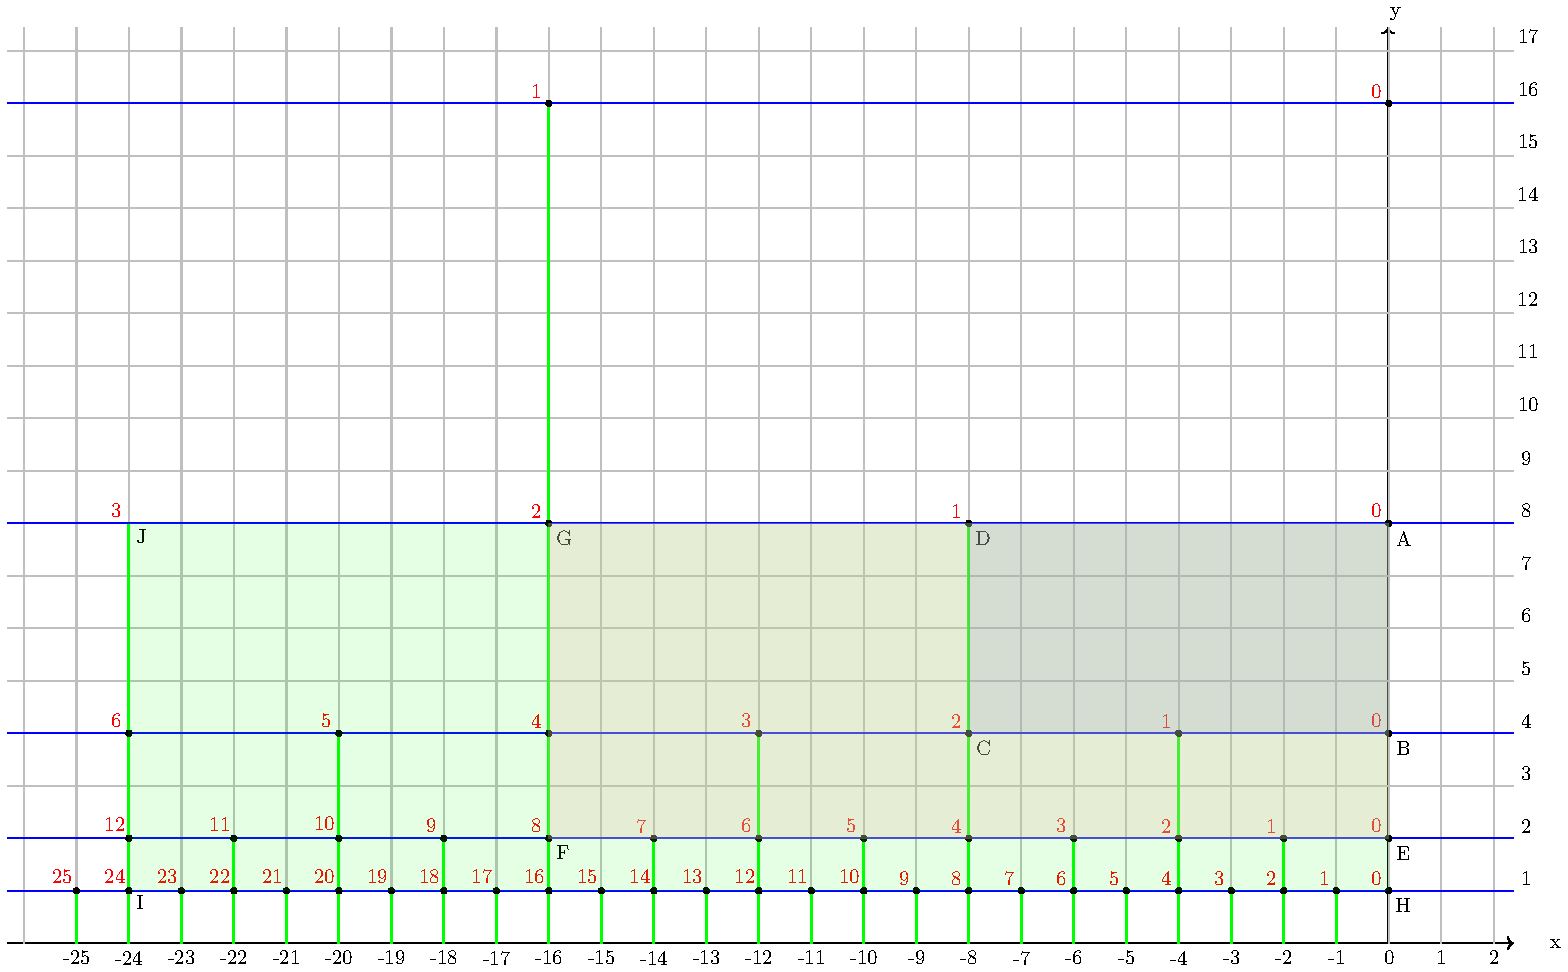
\includegraphics{images/17-area-formula}}
    \caption{Illustration of the correspondence between hyperbolic area and arithmetic torsion}\label{fig:area-formula}
\end{figure}

Figure~\ref{fig:area-formula} illustrates the relationship between the area enclosed by expression paths in the grid and the resulting torsion. Consider the following expression identity comparisons:

\begin{itemize}
    \item One-step case:
    \begin{equation}
        x \times 2 + 1 - (x + 1) \times 2 = -1
    \end{equation}

    \item Two-step case:
    \begin{equation}
        x \times 4 + 2 - (x + 2) \times 4 = -6
    \end{equation}

    \item Three-step case:
    \begin{equation}
        x \times 8 + 3 - (x + 3) \times 8 = -21
    \end{equation}
\end{itemize}

These differences correspond precisely to the hyperbolic areas enclosed between alternative evaluation paths within these specific grid examples:

\begin{itemize}
    \item The region $ABCD$ encompasses 1 unit cell.
    \item The region $AEFG$ encompasses 6 unit cells.
    \item The region $AHIJ$ encompasses 21 unit cells.
\end{itemize}
These examples compellingly suggest that arithmetic torsion accumulates in proportion to the area enclosed by the grid paths, indicating a potential connection between algebraic non-commutativity and geometric surface area.

Further supporting this connection, we established a differential formulation:
\begin{equation}
    d\tau = \mu \lambda\, du\, dv \label{eq:area_formula}
\end{equation}
where $d\tau$ represents the infinitesimal arithmetic torsion, and $du\, dv$ denotes the area element in the $(u, v)$ coordinate system adapted to the grid. This equation provides the precise microscopic law linking infinitesimal torsion to the infinitesimal area element.

However, while we possess both macroscopic observations suggesting a torsion-area relationship (from the scaled grid examples) and the exact microscopic differential law \eqref{eq:area_formula}, the explicit integral theorem rigorously bridging these scales is currently underdeveloped. Formulating how the microscopic torsion density $d\tau$ integrates over a finite region to yield the total accumulated torsion—potentially involving boundary terms in analogy with Stokes' theorem, or relating the total torsion to curvature and topology similarly to the Gauss-Bonnet theorem—remains a key objective for future work.

The analogy with curvature in differential geometry therefore becomes particularly pertinent: just as Gaussian curvature encodes deviation from flatness, arithmetic torsion quantifies deviation from commutativity in arithmetic flow. In this sense, torsion constitutes a measure of the operational significance of evaluation order.

The $\mathfrak{E}_1$ space thus provides a mathematical framework where algebraic non-commutativity manifests as measurable geometric distortion—establishing a novel interpretation of arithmetic structure as a form of discrete curvature. This opens avenues for investigating further geometric invariants such as torsion density, torsion-induced flow bifurcation, and \textbf{realizing} a Gauss–Bonnet-type integral identity for arithmetic surfaces.

\subsection{Tube structure}\label{sec:tubestructure}

In preceding sections, we introduced the first kind arithmetic expression space $\mathfrak{E}_1$ as a geometric realization of arithmetic flow under \textbf{fixed} generator parameters $\mu$ and $\lambda$. However, more complex structures emerge when we consider the entire family of spaces indexed by the parameter $\lambda$ (or potentially both $\mu$ and $\lambda$) and analyze how expression behavior evolves across this family. This naturally leads to the concept of a \emph{tube structure}.

\subsubsection{From Slices to Parameterized Families}\label{subsec:tube_slices}

Each individual $\mathfrak{E}_1$ space, denoted $\mathfrak{E}_1^{(\lambda)}$, can be conceptualized as a single \emph{slice} or \emph{fiber} (in the sense of fiber bundles) within the family of expression spaces indexed by the parameter $\lambda$. Within each slice, the evaluation of arithmetic expressions is realized through traversal along (geodesic) paths, the result is governed by the scalar field $a$, and the flow is determined by the metric tensor corresponding to that slice.

Consider a fixed algebraic structure—for instance, an alternating path (with a fixed internal multiplier) corresponding to a polynomial $P(x)$—and examine how its evaluation result $P(e^\lambda)$ evolves as the tube structure parameter $\lambda$ varies. For each value of $\lambda$, the evaluation $P(e^\lambda)$ corresponds to a point (or more accurately, the assignment value $a$ at that point) within the $\lambda$-slice $\mathfrak{E}_1^{(\lambda)}$. As $\lambda$ varies continuously, these points trace out a continuous trajectory through the family of spaces. We refer to such a trajectory generated by $P$ as a \emph{section} or a \emph{$\lambda$-trajectory}. The collection of all slices corresponding to the allowed $\lambda$ values, along with these structures upon them, together form a new, higher-dimensional entity: the tube structure.

\subsubsection{Tube Structure as Total Space}\label{subsec:tube_total_space}

We define a \textbf{tube structure $\mathcal{T}$} as the \emph{total space} formed by the family of $\mathfrak{E}_1$ spaces indexed by a continuous parameter $\lambda$ (typically $\lambda > 0$), which can be formally written as the disjoint union:
\begin{equation}
\mathcal{T} = \bigsqcup_{\lambda > 0} \mathfrak{E}_1^{(\lambda)}
\end{equation}
This total space needs to be endowed with an appropriate topology (and possibly a differential or fiber bundle structure) to support coherent analysis along the $\lambda$-direction.

In this structure:
\begin{itemize}
    \item The \emph{base space} is the parameter domain $\Lambda$ for $\lambda$ (e.g., $\mathbb{R}^+$).
    \item The \emph{fiber} over each point $\lambda$ in the base space is the geometric expression space $\mathfrak{E}_1^{(\lambda)}$.
    \item Fixed algebraic expression structures (especially those corresponding to polynomials $P(x)$, via the evaluation $P(e^\lambda)$) trace \emph{canonical sections} or $\lambda$-trajectories through $\mathcal{T}$. These sections connect the fibers for different $\lambda$.
\end{itemize}

\subsubsection{Zero Loci and Nodal Evolution}\label{subsec:tube_zeros}

A primary motivation for studying tube structures is to investigate how \emph{zero loci}—the sets of points where an expression evaluates to zero ($a=0$)—evolve with the parameter $\lambda$.

\begin{itemize}
    \item \textbf{In the Tube Structure $\mathcal{T}_1$ based on $\mathfrak{E}_1$}: For the $\mathfrak{E}_1$ space ($a=-x/y$) that we have discussed in detail, the zero locus within \textbf{each slice} $\mathfrak{E}_1^{(\lambda)}$ is always the \textbf{same simple} line: the y-axis ($x=0$). Consequently, in the tube structure $\mathcal{T}_1 = \bigsqcup \mathfrak{E}_1^{(\lambda)}$, the overall zero locus is the trivial hyperplane $x=0$.

    \item \textbf{Outlook for Non-Trivial Spaces}: However, as our research suggests, the simplicity of the zero locus in $\mathfrak{E}_1$ might limit its capacity to explain more complex phenomena (like those observed in knot theory examples). Therefore, there is strong motivation to seek and construct \textbf{"non-trivial" arithmetic expression spaces $\mathfrak{E}_{NT}$}, where a single slice $\mathfrak{E}_{NT}^{(\lambda)}$ might possess \textbf{multiple or morphologically more complex zero lines}. In the tube structures $\mathcal{T}_{NT}$ built from such non-trivial spaces, the zero locus itself could evolve with $\lambda$, potentially exhibiting various interesting phenomena, such as:
    \begin{itemize}
        \item \textbf{Bifurcation}: New zero lines might emerge or merge with existing ones as $\lambda$ varies.
        \item \textbf{Branching}: The zero locus of certain expressions might exhibit multi-valued behavior along the $\lambda$-direction.
        \item \textbf{Topology change}: The overall zero surface might develop handles (genus), singularities, or undergo other changes in its topological structure.
    \end{itemize}
\end{itemize}
The analysis of such complex zero loci and their evolution (potentially within $\mathcal{T}_{NT}$) constitutes a core direction for studying expression dynamics, particularly when considering families of expressions or differential equations involving $\lambda$.

\subsubsection{Investigative Approaches and Outlook}\label{subsec:tube_outlook}

The formalism of tube structures opens up multiple avenues for research in arithmetic expression geometry:

\begin{itemize}
    \item Examining the global properties of zero surfaces (in the general case where they might be non-trivial), such as their genus, regions of curvature concentration, and dependence on the parameter $\lambda$.
    \item Studying the geometric properties of sections $\gamma_P$ corresponding to polynomials $P(e^\lambda)$ within the tube structure, and investigating whether imposing geometric continuity conditions leads to algebraic rigidity.
    \item Exploring the possibility of establishing flow equations across the $\lambda$-family, perhaps defining a notion of \emph{connection} or \emph{parallel transport} between different $\lambda$-slices.
    \item Defining \emph{moduli spaces} of expression geometries as structured fiber bundles over parameter spaces.
\end{itemize}

Ultimately, tube structures provide a mathematical framework wherein the dynamics of arithmetic expressions can be analyzed analogously to field theory. In this analogy, expressions (or their underlying algebraic structures) act as structured sections, while quantities like arithmetic torsion, curvature, and zero loci serve as local or global invariants.
\newpage

\section{The accumulative commutative space}\label{sec:acspace}


\subsection{The construction of the grid $G_0$}\label{sec:construction-of-grids}

To construct the grid described in subsection \ref{sec:meshgrid} and Figure \ref{fig:gridex0},
we will use the number theory decomposition introduced by Victor Pambuccian in \cite{Pambuccian2016THEAO} and
Celia Schacht in \cite{Schacht2018ANOTHERAO}.

$$
n = \tau(n) \omega(n)
$$

where $\tau(n)$ is a power of 2 and $\omega(n)$ is an odd.

We can see directly from the Figure \ref{fig:gridex0} that the grid is constructed by the following rules:
\begin{itemize}
\item horizantal lines (blue, additional lines) satisfying $y = 2^k, k \in \mathbb{Z}$
\item vertical lines (green, multiplicative lines) satisfying
    \begin{itemize}
        \item the value of x satisfying $x = \frac{m}{2^l}, l \in \mathbb{Z}^+, m \in \mathbb{Z}$
        \item the assignment begin from $\omega(-m)$ and increase exponentially by power 2.
    \end{itemize}
\end{itemize}

\begin{figure}[ht]
\centering
\resizebox{0.9\textwidth}{!}{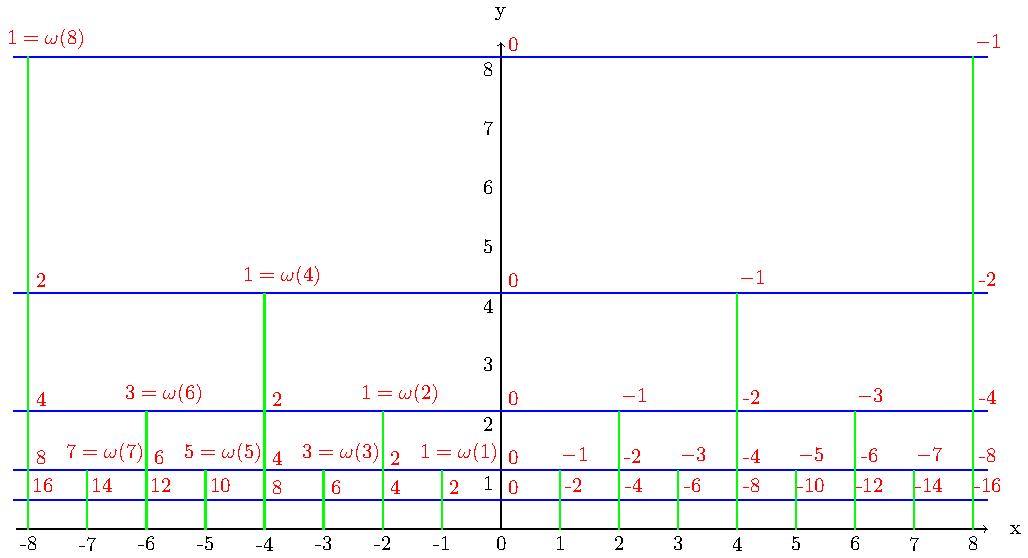
\includegraphics{images/07-grid-detail}}
\caption{$\omega$ gives the assignment at the start points of vertical lines in $G_0$}\label{fig:griddetail}
\end{figure}

The horizontal lines and the vertical lines divide the whole space into a mesh grid $G_0 = (V_0, E_0, F_0)$, where
$V_0$ is the set of crossing points, $E_0$ is the set of edges (segments in the horizontal and vertical lines,
it should be noted that only the vertical lines are geodesics, while the horizontal lines are horocycles) connecting
the crossing points, and $F_0$ is the set of cut cells. This mesh grid is generated by the additional generator $1$ and
the multiplicative generator $2$, and $V_0$, $E_0$, and $F_0$ are all countable sets.

We illustrate the construction schema of $G_0$ in Figure \ref{fig:gridschema}.

\begin{figure}[ht]
\centering
\resizebox{0.9\textwidth}{!}{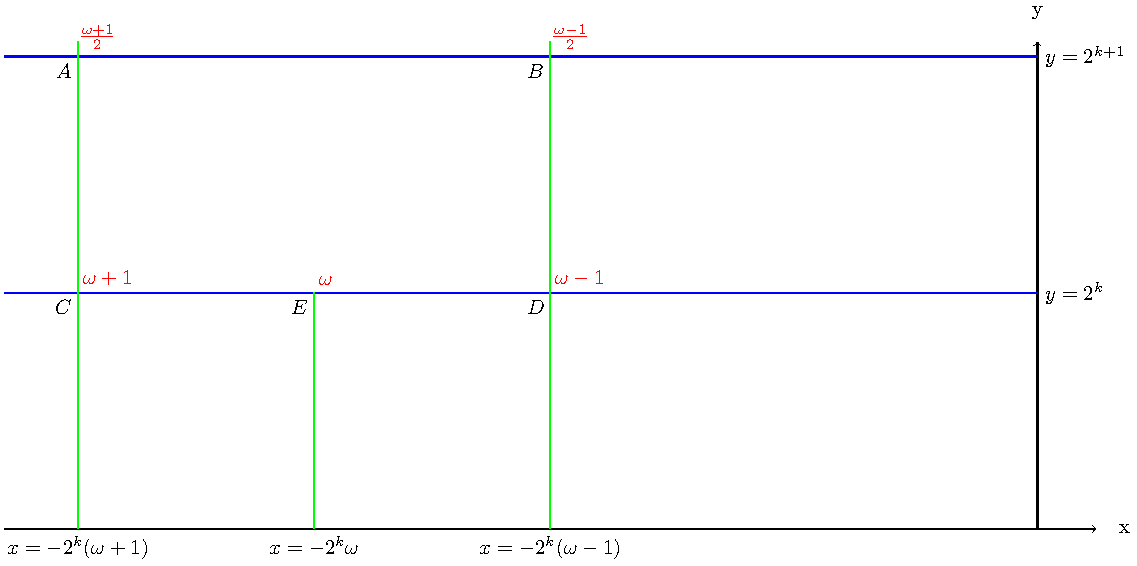
\includegraphics{images/08-grid-schema}}
\caption{the construction schema of $G_0$}\label{fig:gridschema}
\end{figure}

We notice that $G_0$ is very regular, in fact, all edges are equidistant.

\begin{lemma}\label{lem:regular}
All edges in $G_0$ are equidistant.
\end{lemma}

\begin{proof}
Following the construction schema in Figure \ref{fig:gridschema}, we can calculate the length of segments are all equidistant.

Length of $AC$ and $BD$:

$$
\int ds = \int\limits_{2^{k}}^{2^{k+1}} \frac{1}{y \ln 2} dy = \frac{1}{\ln 2} \left( \ln 2^{k+1} - \ln 2^k \right) = 1
$$

Length of $AB$:

$$
\int ds = \int\limits_{-2^k(\omega + 1)}^{-2^k(\omega - 1)} \frac{1}{2^{k+1}} dx = \frac{1}{2^{k+1}} \left( 2^{k + 1} \right) = 1
$$

Length of $CE$:

$$
\int ds = \int\limits_{-2^k(\omega + 1)}^{-2^k \omega} \frac{1}{2^k} dx = \frac{1}{2^k} \left( 2^k \right) = 1
$$

Length of $ED$:

$$
\int ds = \int\limits_{-2^k \omega}^{-2^k(\omega - 1)} \frac{1}{2^k} dx = \frac{1}{2^k} \left( 2^k \right) = 1
$$
\end{proof}

\subsection{The construction of the grid $G_1$}\label{sec:construction-of-grids}

We can similarly construct the grid $G_1$ using the additional generator $\frac{1}{2}$ and the multiplicative generator
$\sqrt{2}$, the grid $G_2$ using the additional generator $\frac{1}{4}$ and the multiplicative generator $\sqrt[4]{2}$,
and so on. And each time the cell of the mesh grid is divided into smaller cells and the end points of the vertical lines
move upward.

\begin{figure}[ht]
\centering
\resizebox{0.9\textwidth}{!}{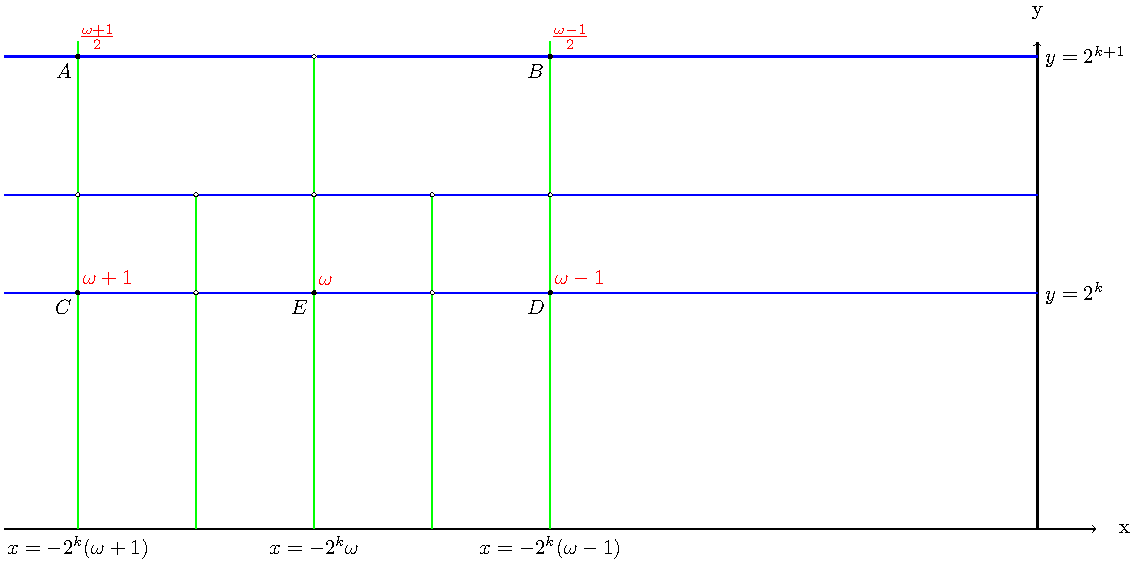
\includegraphics{images/09-grid-schema-g1}}
\caption{the construction schema of $G_1$}\label{fig:gridschemag1}
\end{figure}

\subsection{The construction of the grid $G_2$}\label{sec:construction-of-grids}


\subsection{The grid mesh is dense}\label{sec:construction-of-grids}

It is easy to see that there is a chain of inclusion relations:
$$
V_0 \subset V_1 \subset V_2 \subset \cdots V_i \subset \cdots
$$

Suppose $V = \bigcup_{i=1}^{\infty} V_i$, we have below lemma

\begin{lemma}
$V$ is a countable dense set.
\end{lemma}

\begin{proof}
Because $V_i$ is countable, and the union is over a countable index set, so $V$ is countable.

We can prove it is dense by contradiction. Suppose $V$ is not a dense set. Then there is a point $p$ in the space
neither belongs to $V$ nor is a limit point of $V$.

TODO...

\end{proof}

\subsection{Completeness and topology}\label{sec:topdef}

\subsection{As a special integral}\label{sec:integral}

\newpage

\newpage

%
% \section{Three dimensional constructions}\label{sec:3dconstuction}
%
% In this section, we construct an special domain in the Euclidean plane, and then define a new model for hyperbolic plane based on this domain.
We show that this model is isometric to the Poincar\'e disk model. Finally, we provide two ways to construct the order-4 apeirogonal tiling of the hyperbolic plane.
We also defined three scalar fields $X, Y, L$ on the hyperbolic plane which will be used in the next section.

\subsection{The order-4 Cayley tree $T$}\label{sec:tree}

\begin{figure}
    \centering
    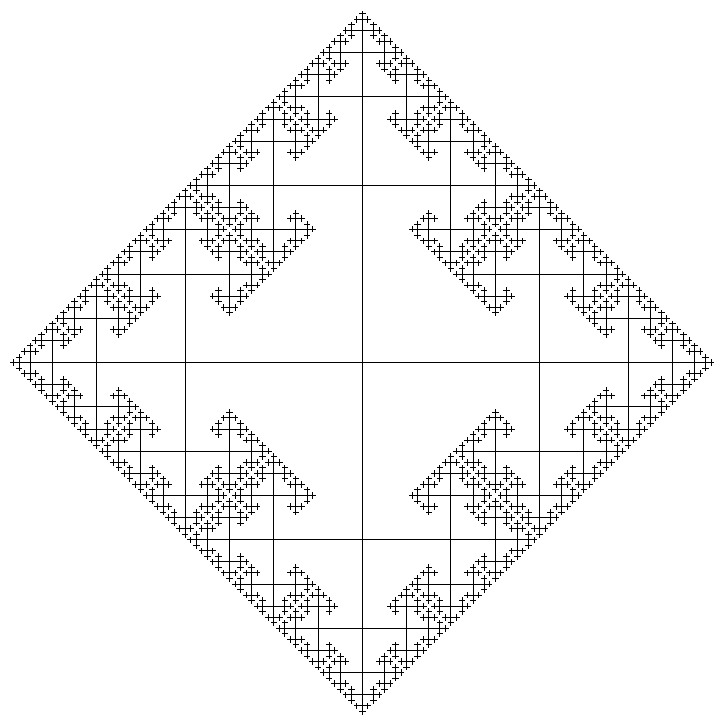
\includegraphics[width=0.6\textwidth]{images/cayley4}
    \caption{The order-4 Cayley tree}
\end{figure}


\subsection{A domain construction based on $T$}\label{sec:domain}

Cut and glue

We define a domain $D$ in the Euclidean plane as follows. Let $D$ be the union of the following regions:

\begin{figure}
    \centering
    
\includegraphics[width=0.2\textwidth]{images/cayley-tree-4-border-2}
    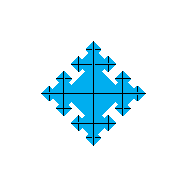
\includegraphics[width=0.2\textwidth]{images/cayley-tree-4-border-3}
    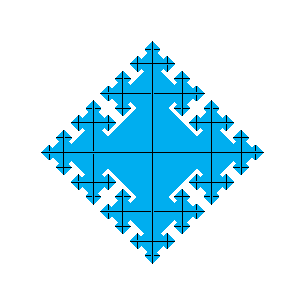
\includegraphics[width=0.2\textwidth]{images/cayley-tree-4-border-4}
    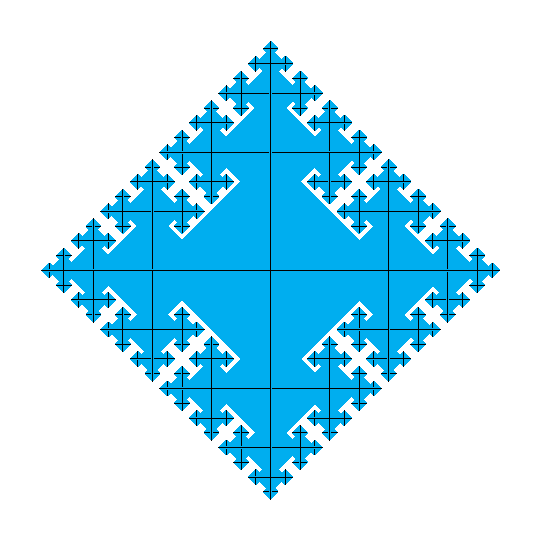
\includegraphics[width=0.2\textwidth]{images/cayley-tree-4-border-5}
    \caption{Construction steps 2, 3, 4, and 5 of the tree $T$ and the domain $D$}
\end{figure}

\subsection{$\mathcal{L}_1$ distance and functions $L, X, Y$ }\label{sec:fields}

\subsection{Cayley model of the hyperbloic plane $\mathbf{H}_2$}\label{sec:model}

\subsection{Order-4 apeirogonal tiling}\label{sec:tilling}


% \newpage
%
% \section{On order-4 apeirogonal tiling}\label{sec:tiling}
%
% In this section, we construct an special domain in the Euclidean plane, and then define a new model for hyperbolic plane based on this domain.
We show that this model is isometric to the Poincar\'e disk model. Finally, we provide two ways to construct the order-4 apeirogonal tiling of the hyperbolic plane.
We also defined three scalar fields $X, Y, L$ on the hyperbolic plane which will be used in the next section.

\subsection{The order-4 Cayley tree $T$}\label{sec:tree}

\begin{figure}
    \centering
    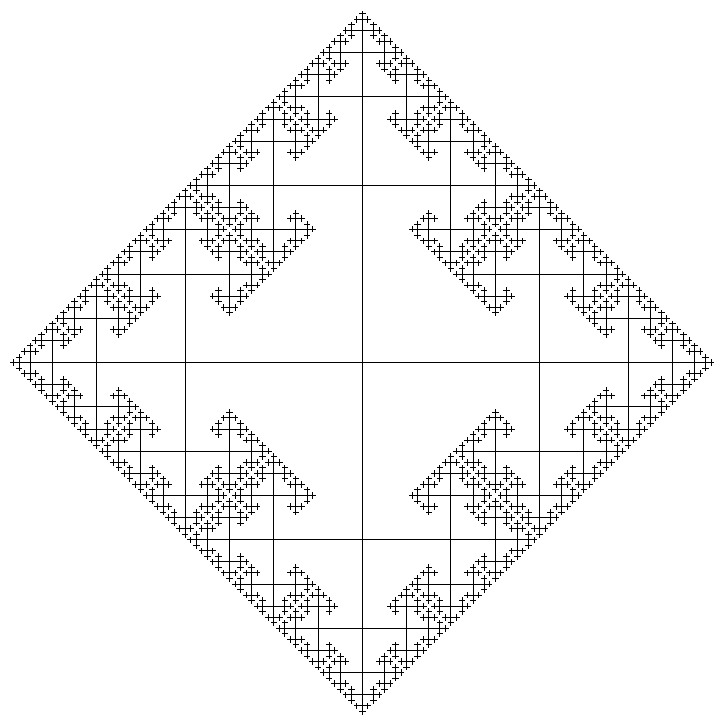
\includegraphics[width=0.6\textwidth]{images/cayley4}
    \caption{The order-4 Cayley tree}
\end{figure}


\subsection{A domain construction based on $T$}\label{sec:domain}

Cut and glue

We define a domain $D$ in the Euclidean plane as follows. Let $D$ be the union of the following regions:

\begin{figure}
    \centering
    
\includegraphics[width=0.2\textwidth]{images/cayley-tree-4-border-2}
    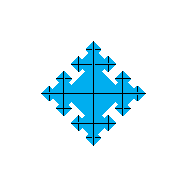
\includegraphics[width=0.2\textwidth]{images/cayley-tree-4-border-3}
    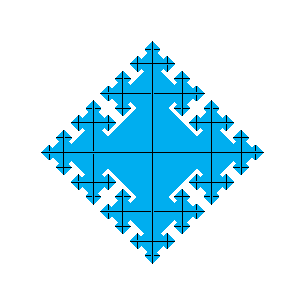
\includegraphics[width=0.2\textwidth]{images/cayley-tree-4-border-4}
    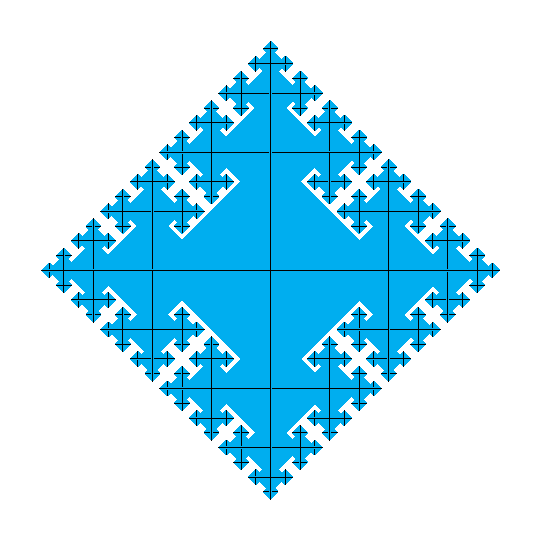
\includegraphics[width=0.2\textwidth]{images/cayley-tree-4-border-5}
    \caption{Construction steps 2, 3, 4, and 5 of the tree $T$ and the domain $D$}
\end{figure}

\subsection{$\mathcal{L}_1$ distance and functions $L, X, Y$ }\label{sec:fields}

\subsection{Cayley model of the hyperbloic plane $\mathbf{H}_2$}\label{sec:model}

\subsection{Order-4 apeirogonal tiling}\label{sec:tilling}


% \newpage
%
% \section{Topological arithmetic expression space}\label{sec:topology}
%
% 
\subsection{Definition and Intuition}
A pair of real-valued functions $(f,g)=(f(u,v,a),g(u,v,a))$ is said to be \textbf{arithmetic holomorphic} if it satisfies the AEG-Cauchy-Riemann equations:
\begin{equation}\label{eq:16}\tag{16}
D_u f=D_v g,\qquad D_v f=-D_u g.
\end{equation}
This definition lifts the classic Cauchy-Riemann conditions from the complex plane $\mathbb{C} \cong \mathbb{R}^2(u,v)$ to the horizontal geometry of the arithmetic expression contact structure.

\subsection{Basic Properties and Proof Sketches}
\begin{enumerate}
    \item \textbf{Conformality and Modulus Equality}: The vectors $(D_uf,D_ug)$ and $(D_vf,D_vg)$ are orthogonal and have equal magnitude:
    \[
    (D_uf)^2+(D_ug)^2=(D_vf)^2+(D_vg)^2.
    \]
    The proof follows from direct substitution using Eq.~\eqref{eq:16}.

    \item \textbf{Closure Properties}: The set of arithmetic holomorphic pairs is closed under addition and an "AEG complex multiplication" defined as $(f,g)\odot(\tilde f,\tilde g)=(f\tilde f- g\tilde g,\ f\tilde g+\tilde f g)$. Furthermore, composition with a classic holomorphic function of $(u,v)$ preserves arithmetic holomorphicity.

    \item \textbf{Classical Limit}: If $f$ and $g$ are independent of $a$, then $D_u=\partial_u$ and $D_v=\partial_v$, and the AEG-CR equations reduce to the standard Cauchy-Riemann equations.

    \item \textbf{Rigidity}: If $f=f(a)$ and $g=g(a)$, the only solutions are constants. (\textit{Hint}: Eq.~\eqref{eq:16} forces the vectors $(f'(a), g'(a))$ and $(\mu, \lambda a)$ to be simultaneously orthogonal and equal in magnitude, which is impossible unless they are zero.)

    \item \textbf{Scaling of the Curvature Density}: In arithmetic holomorphic coordinates $(f,g)$, the curvature 2-form transforms as:
    \begin{equation}\label{eq:17}\tag{17}
    d\omega=\frac{\mu\lambda}{|F'|^2}\,df\wedge dg,\qquad \text{where } |F'|^2:=(D_uf)^2+(D_ug)^2.
    \end{equation}
    The area density scales by the Jacobian factor, but the total integral remains invariant. This provides an area formula for "expression conformal coordinates".
\end{enumerate}

% \newpage
%
% \section{From arithmetic torsion to curvature}\label{sec:curvature}
%
% 
\subsection{The construction of the grid $G_0$}\label{sec:construction-of-grids}

To construct the grid described in subsection \ref{sec:meshgrid} and Figure \ref{fig:gridex0},
we will use the number theory decomposition introduced by Victor Pambuccian in \cite{Pambuccian2016THEAO} and
Celia Schacht in \cite{Schacht2018ANOTHERAO}.

$$
n = \tau(n) \omega(n)
$$

where $\tau(n)$ is a power of 2 and $\omega(n)$ is an odd.

We can see directly from the Figure \ref{fig:gridex0} that the grid is constructed by the following rules:
\begin{itemize}
\item horizantal lines (blue, additional lines) satisfying $y = 2^k, k \in \mathbb{Z}$
\item vertical lines (green, multiplicative lines) satisfying
    \begin{itemize}
        \item the value of x satisfying $x = \frac{m}{2^l}, l \in \mathbb{Z}^+, m \in \mathbb{Z}$
        \item the assignment begin from $\omega(-m)$ and increase exponentially by power 2.
    \end{itemize}
\end{itemize}

\begin{figure}[ht]
\centering
\resizebox{0.9\textwidth}{!}{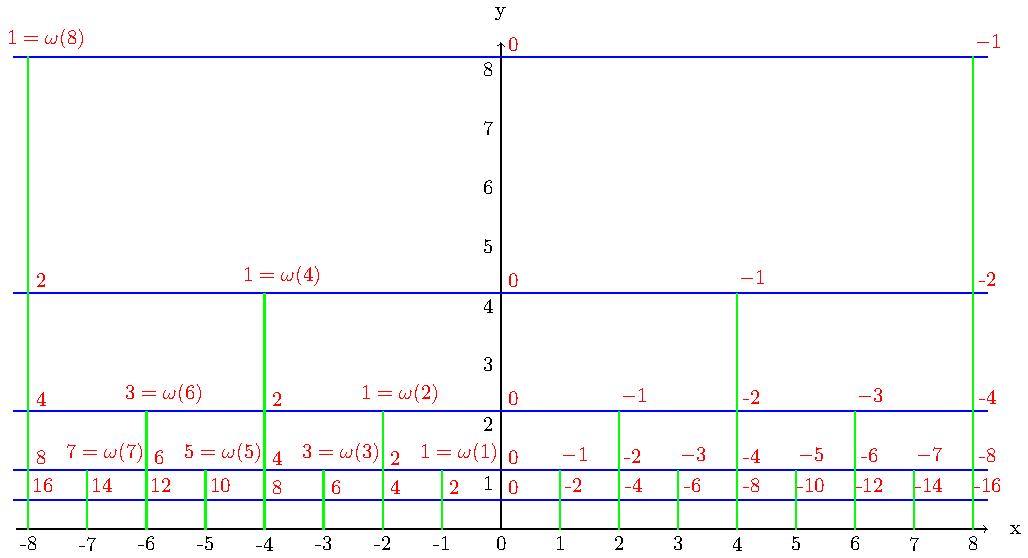
\includegraphics{images/07-grid-detail}}
\caption{$\omega$ gives the assignment at the start points of vertical lines in $G_0$}\label{fig:griddetail}
\end{figure}

The horizontal lines and the vertical lines divide the whole space into a mesh grid $G_0 = (V_0, E_0, F_0)$, where
$V_0$ is the set of crossing points, $E_0$ is the set of edges (segments in the horizontal and vertical lines,
it should be noted that only the vertical lines are geodesics, while the horizontal lines are horocycles) connecting
the crossing points, and $F_0$ is the set of cut cells. This mesh grid is generated by the additional generator $1$ and
the multiplicative generator $2$, and $V_0$, $E_0$, and $F_0$ are all countable sets.

We illustrate the construction schema of $G_0$ in Figure \ref{fig:gridschema}.

\begin{figure}[ht]
\centering
\resizebox{0.9\textwidth}{!}{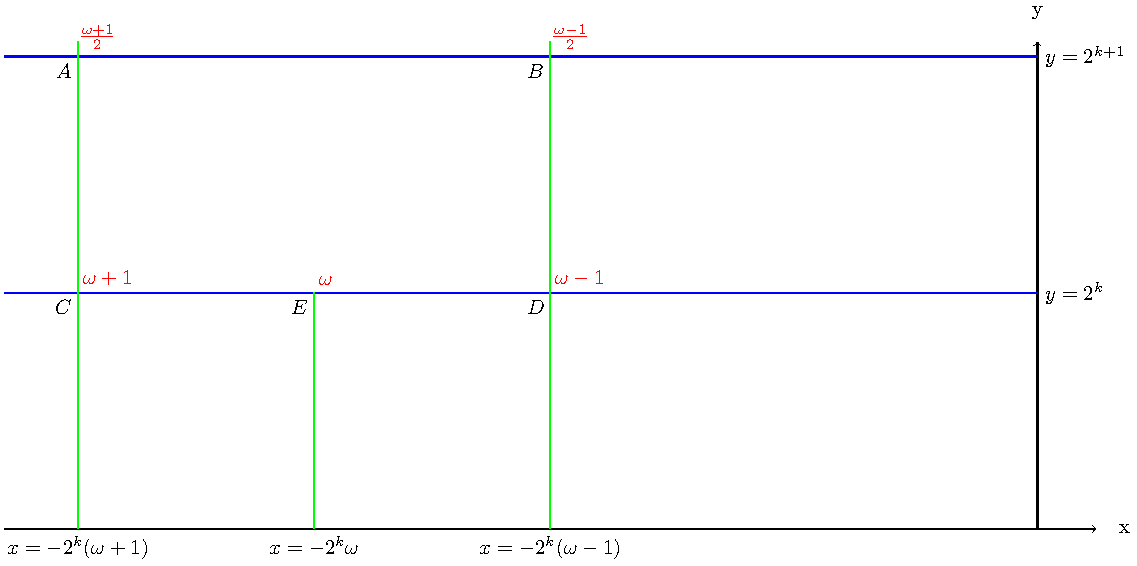
\includegraphics{images/08-grid-schema}}
\caption{the construction schema of $G_0$}\label{fig:gridschema}
\end{figure}

We notice that $G_0$ is very regular, in fact, all edges are equidistant.

\begin{lemma}\label{lem:regular}
All edges in $G_0$ are equidistant.
\end{lemma}

\begin{proof}
Following the construction schema in Figure \ref{fig:gridschema}, we can calculate the length of segments are all equidistant.

Length of $AC$ and $BD$:

$$
\int ds = \int\limits_{2^{k}}^{2^{k+1}} \frac{1}{y \ln 2} dy = \frac{1}{\ln 2} \left( \ln 2^{k+1} - \ln 2^k \right) = 1
$$

Length of $AB$:

$$
\int ds = \int\limits_{-2^k(\omega + 1)}^{-2^k(\omega - 1)} \frac{1}{2^{k+1}} dx = \frac{1}{2^{k+1}} \left( 2^{k + 1} \right) = 1
$$

Length of $CE$:

$$
\int ds = \int\limits_{-2^k(\omega + 1)}^{-2^k \omega} \frac{1}{2^k} dx = \frac{1}{2^k} \left( 2^k \right) = 1
$$

Length of $ED$:

$$
\int ds = \int\limits_{-2^k \omega}^{-2^k(\omega - 1)} \frac{1}{2^k} dx = \frac{1}{2^k} \left( 2^k \right) = 1
$$
\end{proof}

\subsection{The construction of the grid $G_1$}\label{sec:construction-of-grids}

We can similarly construct the grid $G_1$ using the additional generator $\frac{1}{2}$ and the multiplicative generator
$\sqrt{2}$, the grid $G_2$ using the additional generator $\frac{1}{4}$ and the multiplicative generator $\sqrt[4]{2}$,
and so on. And each time the cell of the mesh grid is divided into smaller cells and the end points of the vertical lines
move upward.

\begin{figure}[ht]
\centering
\resizebox{0.9\textwidth}{!}{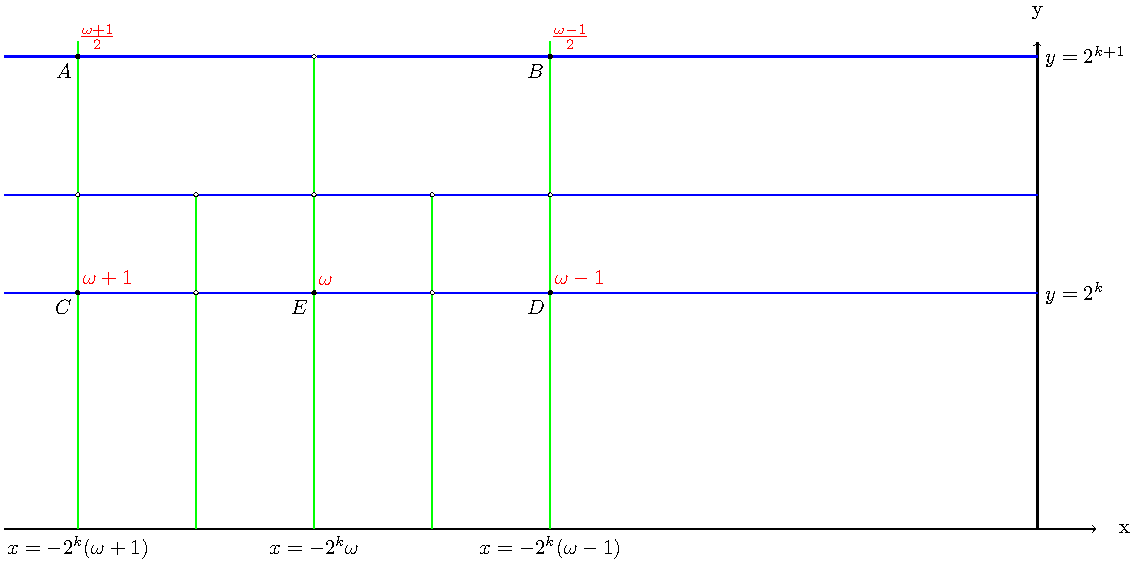
\includegraphics{images/09-grid-schema-g1}}
\caption{the construction schema of $G_1$}\label{fig:gridschemag1}
\end{figure}

\subsection{The construction of the grid $G_2$}\label{sec:construction-of-grids}


\subsection{The grid mesh is dense}\label{sec:construction-of-grids}

It is easy to see that there is a chain of inclusion relations:
$$
V_0 \subset V_1 \subset V_2 \subset \cdots V_i \subset \cdots
$$

Suppose $V = \bigcup_{i=1}^{\infty} V_i$, we have below lemma

\begin{lemma}
$V$ is a countable dense set.
\end{lemma}

\begin{proof}
Because $V_i$ is countable, and the union is over a countable index set, so $V$ is countable.

We can prove it is dense by contradiction. Suppose $V$ is not a dense set. Then there is a point $p$ in the space
neither belongs to $V$ nor is a limit point of $V$.

TODO...

\end{proof}

\subsection{Completeness and topology}\label{sec:topdef}

\subsection{As a special integral}\label{sec:integral}

\newpage

% \newpage
%
% \section{Tube structure, complexification and fibration}\label{sec:morekinds}
%
% 
\subsection{On integral theory}\label{sec:integral}

\subsection{On representation of function}\label{sec:function}

\subsection{Questions related with complexity?}\label{sec:complexity}

% \newpage
%
% \section{General discussion}\label{sec:function}
%
% 
\subsection{On integral theory}\label{sec:integral}

\subsection{On representation of function}\label{sec:function}

\subsection{Questions related with complexity?}\label{sec:complexity}

% \newpage

% \section{A glossary of unsolved problems}\label{sec:problems}
%
% 
We can also get a direct formal solution of the flow equation (\eqref{eq:flow}) step by step:

$$
    \frac{da}{\mu \cos \theta + a \lambda \sin \theta} = ds
$$

$$
    \frac{1}{\lambda \sin \theta} \frac{d(\mu \cos \theta + a \lambda \sin \theta)}{\mu \cos \theta + a \lambda \sin \theta} = ds
$$

$$
    \frac{1}{\lambda \sin \theta} ln(\mu \cos \theta + a \lambda \sin \theta) = s + C
$$

$$
    \mu \cos \theta + a \lambda \sin \theta = e^{\lambda s \sin \theta} e^{C \lambda \sin \theta}
$$

Considering the initial condition
$$
    \mu \cos \theta + a_0 \lambda \sin \theta = e^{C \lambda \sin \theta}
$$

We have
$$
    \mu \cos \theta + a \lambda \sin \theta = e^{\lambda s \sin \theta} (\mu \cos \theta + a_0 \lambda \sin \theta)
$$

$$
   a = \frac{\mu \cos \theta + a_0 \lambda \sin \theta}{\lambda \sin \theta} e^{\lambda s \sin \theta} - \frac{\mu}{\lambda}\cot \theta
$$

$$
   a = (a_0 + \frac{\mu}{\lambda} \cot \theta) e^{\lambda s \sin \theta} - \frac{\mu}{\lambda} \cot \theta
$$

\begin{equation}
   a =  a_0 e^{\lambda s \sin \theta} + \frac{\mu}{\lambda} (e^{\lambda s \sin \theta} - 1) \cot \theta
\end{equation}

\begin{equation}\label{eq:directformalsolution}
   a =  a_0 e^{\lambda s \sin \theta} + \frac{\mu}{\lambda} (e^{\lambda s \sin \theta} - 1) \cot \theta
\end{equation}


% \newpage

\bibliographystyle{plain}
\bibliography{aeg-paper.bib}
\newpage

\appendix

\section{Solution of the flow equation}\label{sec:directformalsolution}


We can also get a direct formal solution of the flow equation (\eqref{eq:flow}) step by step:

$$
    \frac{da}{\mu \cos \theta + a \lambda \sin \theta} = ds
$$

$$
    \frac{1}{\lambda \sin \theta} \frac{d(\mu \cos \theta + a \lambda \sin \theta)}{\mu \cos \theta + a \lambda \sin \theta} = ds
$$

$$
    \frac{1}{\lambda \sin \theta} ln(\mu \cos \theta + a \lambda \sin \theta) = s + C
$$

$$
    \mu \cos \theta + a \lambda \sin \theta = e^{\lambda s \sin \theta} e^{C \lambda \sin \theta}
$$

Considering the initial condition
$$
    \mu \cos \theta + a_0 \lambda \sin \theta = e^{C \lambda \sin \theta}
$$

We have
$$
    \mu \cos \theta + a \lambda \sin \theta = e^{\lambda s \sin \theta} (\mu \cos \theta + a_0 \lambda \sin \theta)
$$

$$
   a = \frac{\mu \cos \theta + a_0 \lambda \sin \theta}{\lambda \sin \theta} e^{\lambda s \sin \theta} - \frac{\mu}{\lambda}\cot \theta
$$

$$
   a = (a_0 + \frac{\mu}{\lambda} \cot \theta) e^{\lambda s \sin \theta} - \frac{\mu}{\lambda} \cot \theta
$$

\begin{equation}
   a =  a_0 e^{\lambda s \sin \theta} + \frac{\mu}{\lambda} (e^{\lambda s \sin \theta} - 1) \cot \theta
\end{equation}

\begin{equation}\label{eq:directformalsolution}
   a =  a_0 e^{\lambda s \sin \theta} + \frac{\mu}{\lambda} (e^{\lambda s \sin \theta} - 1) \cot \theta
\end{equation}


\newpage

% \section{Infinitesimal-discrete conformance}\label{sec:conformance}
%
% 
In order to verify the conformance, we expand the formula \eqref{eq:directformalsolution} in the following way:

\begin{equation}
   a =  a_0 e^{\lambda s \sin \theta} + \frac{\mu}{\lambda} [1 + \lambda s \sin \theta + \frac{1}{2!} (\lambda s \sin \theta)^2  + \frac{1}{3!} (\lambda s \sin \theta)^3 + \cdots - 1] \cot \theta
\end{equation}

\begin{equation}
   a = a_0 e^{\lambda s \sin \theta} + \mu s \cos \theta + \frac{\mu}{\lambda} \sin \theta \cos \theta (\frac{\lambda^2s^2}{2!} + \frac{\lambda^3s^3}{3!} \sin \theta + \frac{\lambda^4s^4}{4!} \sin^2 \theta + \cdots)
\end{equation}

\begin{equation}
   a = a_0 e^{\lambda s \sin \theta} + \mu s \cos \theta + \frac{\mu}{2\lambda} \sin 2\theta (\frac{\lambda^2s^2}{2!} + \frac{\lambda^3s^3}{3!} \sin \theta + \frac{\lambda^4s^4}{4!} \sin^2 \theta + \cdots)
\end{equation}

\begin{equation}
   a = a_0 e^{\lambda s \sin \theta} + \mu s \cos \theta + \frac{\mu}{2\lambda} \Psi(s) \sin 2\theta
\end{equation}

When $\theta = \frac{k \pi}{2}, k = 0, 1, 2, 3\cdots, s = 0, 1, 2, 3\cdots$, we have

\begin{equation}
    a = a_0 e^{\lambda s \sin \theta} + \mu s \cos \theta
\end{equation}

Especially, we have

\begin{equation}
    a = a_0 + \mu s, s = 0, 1, 2, 3\cdots, k = 0, 1, 2, 3\cdots, \theta = 2k\pi
\end{equation}

\begin{equation}
    a = x_0e^{\lambda s}, s = 0, 1, 2, 3\cdots, k = 0, 1, 2, 3\cdots, \theta = 2k\pi + \frac{\pi}{2}
\end{equation}

\begin{equation}
    a = a_0 - \mu s, s = 0, 1, 2, 3\cdots, k = 0, 1, 2, 3\cdots, \theta = 2k\pi + \pi
\end{equation}

\begin{equation}
    a = a_0 e^{- \lambda s}, s = 0, 1, 2, 3\cdots, k = 0, 1, 2, 3\cdots, \theta = 2k\pi + \frac{3 \pi}{2}
\end{equation}

which gives the conformance.


% \newpage

\section{Geometry calculation}\label{sec:geometrycalculationn}


\subsection{Curvature}\label{sec:curvature-calculations}

Giving

\[
    ds^2 = \frac{1}{y^2} (\frac{dx^2}{\mu^2} + \frac{dy^2}{\lambda^2})
\]

in order to calculate the curvature $K$, we follow the equations in text book

\[
    K = - \frac{1}{A B} \left(\partial_y \left(\frac{\partial_y A}{B}\right) + \partial_x \left(\frac{\partial_x B}{A}\right)\right)
\]

where

\[
    A = \frac{1}{\mu y}, \quad B = \frac{1}{\lambda y}
\]

so we have

\[
    K = - \mu \lambda y^2 \left(
          \partial_y \left(\lambda y \partial_y \left(\frac{1}{\mu y}\right)\right)
        + \partial_x \left(\mu y \partial_x \left(\frac{1}{\lambda y}\right)\right)
    \right)
\]

\[
    K = - \lambda^2 y^2 \left(
    \partial_y \left( y \partial_y \left(\frac{1}{y} \right)\right)
    \right)
\]

\[
    K = - \lambda^2 y^2 \frac{1}{y^2}
\]

\[
    K = - \lambda^2
\]

\subsection{Area element}\label{sec:area-element}

The area element is given by

\[
    dS = A B dx dy
\]

\textbf{i.e}

\[
    dS = \frac{1}{\mu \lambda y^2} dx dy
\]

\subsection{Arithmetic torsion}\label{sec:torsion-calculations}

The arithmetic torsion is given by
\[
    \tau = \mu \lambda dS = \frac{1}{y^2}
\]

\subsection{Laplacian}\label{sec:laplacian-calculations}

\newpage

\newpage

% \section{Grid calculation}\label{sec:gridcalculation}
%
% 
\subsection{Arc length}\label{sec:arclength}

\subsection{Perimeter}\label{sec:perimeter}

\subsection{Area}\label{sec:area}

\subsection{Arithmetic torsion}\label{sec:torsion}

\newpage

% \newpage

% \section{Arithmetic expression, combinators and transformation over trees}\label{sec:expressions}
%
% 
\subsection{LISP and combinators}\label{sec:donaghey}

\subsection{Applicative and concatenative}\label{sec:donaghey}

\subsection{Donaghey transformation}\label{sec:donaghey}

\newpage

% \newpage

\end{document}
